\documentclass[a4paper,12pt,twoside]{memoir}

\usepackage{verbatim} % mlb0029 Para \begin{comment}
\setlength\epigraphwidth{.8\textwidth}
\setlength\epigraphrule{0pt}

% Castellano
\usepackage[spanish,es-tabla]{babel}
\selectlanguage{spanish}
\usepackage[utf8]{inputenc}
\usepackage[T1]{fontenc}
\usepackage{lmodern} % Scalable font
\usepackage{microtype}
\usepackage{placeins}

\usepackage{graphicx}
\usepackage{subcaption}
\usepackage[numbers,sort]{natbib}

\RequirePackage{booktabs}
\RequirePackage[table]{xcolor}
\RequirePackage{xtab}
\RequirePackage{multirow}

% Links
\PassOptionsToPackage{hyphens}{url}\usepackage[colorlinks, breaklinks]{hyperref} %\PassOptionsToPackage{hyphens}{url} para cortar url largas https://tex.stackexchange.com/questions/3033/forcing-linebreaks-in-url
\hypersetup{
	colorlinks,
	allcolors = {red}
}

% Ecuaciones
\usepackage{amsmath}

% Rutas de fichero / paquete
\newcommand{\ruta}[1]{{\sffamily #1}}

% Párrafos
\nonzeroparskip


% Imagenes
\usepackage{graphicx}
\newcommand{\imagen}[2]{
	\begin{figure}[!h]
		\centering
		\includegraphics[width=0.9\textwidth]{#1}
		\caption{#2}\label{fig:#1}
	\end{figure}
	\FloatBarrier
}

\usepackage{listings}

\newcommand{\imagenflotante}[2]{
	\begin{figure}%[!h]
		\centering
		\includegraphics[width=0.9\textwidth]{#1}
		\caption{#2}\label{fig:#1}
	\end{figure}
}



% El comando \figura nos permite insertar figuras comodamente, y utilizando
% siempre el mismo formato. Los parametros son:
% 1 -> Porcentaje del ancho de página que ocupará la figura (de 0 a 1)
% 2 --> Fichero de la imagen
% 3 --> Texto a pie de imagen
% 4 --> Etiqueta (label) para referencias
% 5 --> Opciones que queramos pasarle al \includegraphics
% 6 --> Opciones de posicionamiento a pasarle a \begin{figure}
\newcommand{\figuraConPosicion}[6]{%
  \setlength{\anchoFloat}{#1\textwidth}%
  \addtolength{\anchoFloat}{-4\fboxsep}%
  \setlength{\anchoFigura}{\anchoFloat}%
  \begin{figure}[#6]
    \begin{center}%
      \Ovalbox{%
        \begin{minipage}{\anchoFloat}%
          \begin{center}%
            \includegraphics[width=\anchoFigura,#5]{#2}%
            \caption{#3}%
            \label{#4}%
          \end{center}%
        \end{minipage}
      }%
    \end{center}%
  \end{figure}%
}

%
% Comando para incluir imágenes en formato apaisado (sin marco).
\newcommand{\figuraApaisadaSinMarco}[5]{%
  \begin{figure}%
    \begin{center}%
    \includegraphics[angle=90,height=#1\textheight,#5]{#2}%
    \caption{#3}%
    \label{#4}%
    \end{center}%
  \end{figure}%
}
% Para las tablas
\newcommand{\otoprule}{\midrule [\heavyrulewidth]}
%
% Nuevo comando para tablas pequeñas (menos de una página).
\newcommand{\tablaSmall}[5]{%
 \begin{table}
  \begin{center}
   \rowcolors {2}{gray!35}{}
   \begin{tabular}{#2}
    \toprule
    #4
    \otoprule
    #5
    \bottomrule
   \end{tabular}
   \caption{#1}
   \label{tabla:#3}
  \end{center}
 \end{table}
}

%
% Nuevo comando para tablas pequeñas (menos de una página).
\newcommand{\tablaSmallSinColores}[5]{%
 \begin{table}[H]
  \begin{center}
   \begin{tabular}{#2}
    \toprule
    #4
    \otoprule
    #5
    \bottomrule
   \end{tabular}
   \caption{#1}
   \label{tabla:#3}
  \end{center}
 \end{table}
}

\newcommand{\tablaApaisadaSmall}[5]{%
\begin{landscape}
  \begin{table}
   \begin{center}
    \rowcolors {2}{gray!35}{}
    \begin{tabular}{#2}
     \toprule
     #4
     \otoprule
     #5
     \bottomrule
    \end{tabular}
    \caption{#1}
    \label{tabla:#3}
   \end{center}
  \end{table}
\end{landscape}
}

%
% Nuevo comando para tablas grandes con cabecera y filas alternas coloreadas en gris.
\newcommand{\tabla}[6]{%
  \begin{center}
    \tablefirsthead{
      \toprule
      #5
      \otoprule
    }
    \tablehead{
      \multicolumn{#3}{l}{\small\sl continúa desde la página anterior}\\
      \toprule
      #5
      \otoprule
    }
    \tabletail{
      \hline
      \multicolumn{#3}{r}{\small\sl continúa en la página siguiente}\\
    }
    \tablelasttail{
      \hline
    }
    \bottomcaption{#1}
    \rowcolors {2}{gray!35}{}
    \begin{xtabular}{#2}
      #6
      \bottomrule
    \end{xtabular}
    \label{tabla:#4}
  \end{center}
}

%
% Nuevo comando para tablas grandes con cabecera.
\newcommand{\tablaSinColores}[6]{%
  \begin{center}
    \tablefirsthead{
      \toprule
      #5
      \otoprule
    }
    \tablehead{
      \multicolumn{#3}{l}{\small\sl continúa desde la página anterior}\\
      \toprule
      #5
      \otoprule
    }
    \tabletail{
      \hline
      \multicolumn{#3}{r}{\small\sl continúa en la página siguiente}\\
    }
    \tablelasttail{
      \hline
    }
    \bottomcaption{#1}
    \begin{xtabular}{#2}
      #6
      \bottomrule
    \end{xtabular}
    \label{tabla:#4}
  \end{center}
}

%
% Nuevo comando para tablas grandes sin cabecera.
\newcommand{\tablaSinCabecera}[5]{%
  \begin{center}
    \tablefirsthead{
      \toprule
    }
    \tablehead{
      \multicolumn{#3}{l}{\small\sl continúa desde la página anterior}\\
      \hline
    }
    \tabletail{
      \hline
      \multicolumn{#3}{r}{\small\sl continúa en la página siguiente}\\
    }
    \tablelasttail{
      \hline
    }
    \bottomcaption{#1}
  \begin{xtabular}{#2}
    #5
   \bottomrule
  \end{xtabular}
  \label{tabla:#4}
  \end{center}
}



\definecolor{cgoLight}{HTML}{EEEEEE}
\definecolor{cgoExtralight}{HTML}{FFFFFF}

%
% Nuevo comando para tablas grandes sin cabecera.
\newcommand{\tablaSinCabeceraConBandas}[5]{%
  \begin{center}
    \tablefirsthead{
      \toprule
    }
    \tablehead{
      \multicolumn{#3}{l}{\small\sl continúa desde la página anterior}\\
      \hline
    }
    \tabletail{
      \hline
      \multicolumn{#3}{r}{\small\sl continúa en la página siguiente}\\
    }
    \tablelasttail{
      \hline
    }
    \bottomcaption{#1}
    \rowcolors[]{1}{cgoExtralight}{cgoLight}

  \begin{xtabular}{#2}
    #5
   \bottomrule
  \end{xtabular}
  \label{tabla:#4}
  \end{center}
}

% TODO
%\def\todo{{\color{red}Comentario de revisión...}}

\graphicspath{ {./img/} }

% Capítulos
\chapterstyle{bianchi}
\newcommand{\capitulo}[2]{
	\setcounter{chapter}{#1}
	\setcounter{section}{0}
	\chapter*{#2}
	\addcontentsline{toc}{chapter}{#2}
	\markboth{#2}{#2}
}

% Apéndices
\renewcommand{\appendixname}{Apéndice}
\renewcommand*\cftappendixname{\appendixname}

\newcommand{\apendice}[1]{
	%\renewcommand{\thechapter}{A}
	\chapter{#1}
}

\renewcommand*\cftappendixname{\appendixname\ }

% Formato de portada
\makeatletter
\usepackage{xcolor}
\newcommand{\tutor}[1]{\def\@tutor{#1}}
\newcommand{\course}[1]{\def\@course{#1}}
\definecolor{cpardoBox}{HTML}{E6E6FF}
\def\maketitle{
  \null
  \thispagestyle{empty}
  % Cabecera ----------------
\noindent
\includegraphics[width=\textwidth]{cabecera}\vspace{1cm}%
  \vfill
  % Título proyecto y escudo informática ----------------
  \colorbox{cpardoBox}{%
    \begin{minipage}{.8\textwidth}
      \vspace{.5cm}\Large
      \begin{center}
      \textbf{TFG del Grado en Ingeniería Informática}\vspace{.6cm}\\
      \textbf{\LARGE\@title{}}
      \end{center}
      \vspace{.2cm}
    \end{minipage}

  }%
  \hfill\begin{minipage}{.20\textwidth}
    
\includegraphics[width=\textwidth]{escudoInfor}
  \end{minipage}
  \vfill
  % Datos de alumno, curso y tutores ------------------
  \begin{center}%
  {%
    \noindent\LARGE
    Presentado por \@author{}\\ 
    en Universidad de Burgos --- \@date{}\\
    Tutor: \@tutor{}\\
  }%
  \end{center}%
  \null
  \cleardoublepage
  }
\makeatother

\newcommand{\nombre}{Miguel Ángel León Bardavío} %%% cambio de comando

% Datos de portada
\title{{\Huge Evolution Metrics Gauge}\\[0.5cm]Comparador de métricas de evolución en repositorios software}
\author{\nombre}
\tutor{Carlos López Nozal}
\date{16 de septiembre de 2019}

\begin{document}

\maketitle


\newpage\null\thispagestyle{empty}\newpage


%%%%%%%%%%%%%%%%%%%%%%%%%%%%%%%%%%%%%%%%%%%%%%%%%%%%%%%%%%%%%%%%%%%%%%%%%%%%%%%%%%%%%%%%
\thispagestyle{empty}


\noindent
\includegraphics[width=\textwidth]{cabecera}\vspace{1cm}

\noindent D. Carlos López Nozal, profesor del departamento de Ingeniería Civil, Área de Lenguajes y Sistemas Informáticos.

\noindent Expone:

\noindent Que el alumno D. \nombre, con DNI 71362165L, ha realizado el Trabajo final de Grado en Ingeniería Informática titulado \textit{Comparador de métricas de evolución en repositorios software}. 

\noindent Y que dicho trabajo ha sido realizado por el alumno bajo la dirección del que suscribe, en virtud de lo cual se autoriza su presentación y defensa.

\begin{center} %\large
En Burgos, {\large \today}
\end{center}

\vfill\vfill\vfill

%% Author and supervisor
%\begin{minipage}{0.45\textwidth}
%\begin{flushleft} %\large
%Vº. Bº. del Tutor:\\[2cm]
%D. Carlos López Nozal
%\end{flushleft}
%\end{minipage}
%\hfill
%%\begin{minipage}{0.45\textwidth}
%%\begin{flushleft} %\large
%%Vº. Bº. del co-tutor:\\[2cm]
%%D. nombre co-tutor
%%\end{flushleft}
%%\end{minipage}
%\hfill
%
%\vfill

% para casos con solo un tutor comentar lo anterior
% y descomentar lo siguiente
%Vº. Bº. del Tutor:\\[2cm]
%D. nombre tutor
%Adaptación mlb0029
\begin{minipage}{1\textwidth}
\begin{center} %\large
Vº. Bº. del Tutor:\\[2cm]
D. Carlos López Nozal
\end{center}
\end{minipage}

\newpage\null\thispagestyle{empty}\newpage




\frontmatter

% Abstract en castellano
\renewcommand*\abstractname{Resumen}
\begin{abstract}
%\todo  explicar brevemente  proceso software y su relación con los repositorios de software. Métricas de evolución. ¿qué hace el trabajo? y algun resultado
%\todo Como versión inicial que necesita ser ajustado   añado idea de de un artículo  titulado Emerging topics in mining software repositories.
El proceso del software es un conjunto de actividades cuya meta es el desarrollo o evolución de software. Algunos ejemplos de estas actividades son: la especificación, el diseño, la implementación, pruebas, el aseguramiento de calidad, la configuración del proyecto, etc. 

Los repositorios de código, además de almacenar el código fuente de un proyecto software, pueden incluir sistemas que faciliten las actividades del proceso de software: sistemas de control de versiones, sistemas de seguimiento de incidencias, sistemas de revisión de código, sistemas de despliegue de ejecutables, etc. En la última década han surgido forjas de repositorios que permiten alojar múltiples proyectos, estas son útiles tanto para proyectos empresariales como para proyectos open source.

%\todo Reducir párrafo en inglés
%A software process is a set of related acti\-vi\-ties that culminates in the production of a software package: specification, design, implementation, testing, evolution into new versions, and maintenance. There are also other supporting activities such as configuration and change management, quality assurance, project management, evaluation of user experience, etc. Software repositories are infrastructures to support all these activities. They can be composed with several systems that include code change management, bug tracking, code review, build system, release binaries, wikis, forums, etc. 
Las métricas de evolución ayudan a cuantificar características de los procesos software. Un ejemplo de este tipo de medidas es el \textit{número de días de cierre}, en la que se mide el numero de días que pasan desde que se abre una incidencia hasta su cierre. Estas métricas se pueden obtener gracias a los datos estadísticos que proporcionan los repositorios. 

En este TFG se diseña \textit{\textbf{Evolution Metrics Gauge}}, un software para calcular métricas de evolución sobre distintos repositorios. En el diseño se ha optado por implementar una aplicación Web en Java que toma como entrada un conjunto de repositorios públicos o privados de GitLab y calcula métricas de evolución que permiten comparar los proyectos. Además, se ha procurado un diseño extensible a otras forjas de repositorios y a nuevas métricas. La aplicación ha sido probada con Trabajos Fin de Grado presentados en la Universidad de Burgos y que han sido almacenados en repositorios públicos de GitLab.

Enlace al repositorio del proyecto:
\url{https://gitlab.com/mlb0029/comparador-de-metricas-de-evolucion-en-repositorios-software}

\end{abstract}

\renewcommand*\abstractname{Descriptores}
\begin{abstract}
Métricas de evolución, repositorios de código, proceso de desarrollo de software, ciclo de vida de desarrollo de software, gestión de calidad, forjas de repositorios, comparación de proyectos software, aplicación Web.
\end{abstract}

\clearpage

% Abstract en inglés
\renewcommand*\abstractname{Abstract}
\begin{abstract}

%\todo Idem resumen en español

The software process is a set of activities whose goal is the development or evolution of software. Some examples of these activities are: specification, design, implementation, testing, quality assurance, project management, etc.

The source code repositories, in addition to storing the source code of a software project, may include systems that ease the activities of the software development process: version control systems, issue tracking systems, code review systems, deployment systems, etc. Forges of source code repositories have emerged in the last decade that allow hosting multiple projects, these are useful for both business projects and open-source projects.

Evolution metrics helps to quantify features of a software development process. An example of this type of measure is the \textit {days to close an issue}, in which the number of days that pass from when an incident is opened until its closure is measured. These metrics can be obtained from the statistics provided by the source code repositories.

In this project, \textit{\textbf{Evolution Metrics Gauge}} Web application is designed to calculate evolution metrics on different source code repositories. The design has chosen to implement a Web application in Java language that takes as input a set of GitLab public or private repositories and calculates evolution metrics that allow the repositories to be compared. In addition, an extensible design to other repositories forges and new metrics has been sought. The application has been tested with Final Degree Projects presented at the University of Burgos and that have been stored in public repositories of GitLab.

Link to the project repository:
\url{https://gitlab.com/mlb0029/comparador-de-metricas-de-evolucion-en-repositorios-software}

\end{abstract}

\renewcommand*\abstractname{Keywords}
\begin{abstract}
Evolution metrics, source code repositories, software development process, software development life cycle, quality management, forge of repositories, comparison of software projects, Web application.
\end{abstract}

\clearpage

% Indices
\tableofcontents

\clearpage

\listoffigures

\clearpage

%mlb0029 - No hay tablas
%\listoftables
%\clearpage

\mainmatter
\capitulo{1}{Introducción}

%Descripción del contenido del trabajo y del estrucutra de la memoria y del resto de materiales entregados.

 %\imagen{M1-CalidadProcesos}{Calidad basada en procesos}
\begin{quotation}
	\label{q:Sommerville}
	Una suposición subyacente de la administración de la calidad es que la calidad del proceso de desarrollo afecta directamente a la calidad de los productos a entregar \citep[pág 543]{sommerville_ingenierisoftware_2002}.
\end{quotation}
  \imagen{M1-CalidadProcesos}{Aseguramiento de la calidad basada  en procesos}
  
La calidad del proceso es uno de los factores que determinan la calidad del producto software, tal y como expone Sommerville en la figura \ref{fig:M1-FactoresCalidad}.
\imagen{M1-FactoresCalidad}{Principales factores de calidad del producto de software\cite[pág 561]{sommerville_ingenierisoftware_2002}}
Por esa razón, este trabajo se centra en crear un registro de medidas de proceso de proyectos software alojados en GitLab para, posteriormente, evaluarlos en relación con otros proyectos.

\section{Estructura de la memoria}

La memoria se estructura de la siguiente manera\footnote{\url{https://github.com/ubutfgm/plantillaLatex}}\cite{ubu_plantilla_2019}:

\begin{description}
	\tightlist
	\item[Introducción.] Introducción al trabajo realizado, estructura de la memoria y listado de materiales adjuntos.
	\item[Objetivos del proyecto.] Objetivos que se persiguen alcanzar con la realización del proyecto.
	\item[Conceptos teóricos.] Conceptos clave para comprender los objetivos, el proceso y el producto del proyecto.
	\item[Técnicas y herramientas.] Técnicas y herramientas utilizadas durante el desarrollo del proyecto.
	\item[Aspectos relevantes del desarrollo.] Aspectos destacables durante el proceso de desarrollo del proyecto.
	\item[Trabajos relacionados.] Otros proyectos de la misma naturaleza y los cuales han ayudado a la realización de este.
	\item[Conclusiones y líneas de trabajo futuras.] Conclusiones tras la realización del proyecto y posibilidades de mejora o expansión.
\end{description}

Se incluyen también los siguientes anexos:

\begin{description}
	\tightlist
	\item[Plan del proyecto software.] Planificación temporal y estudio de la viabilidad del proyecto.
	\item[Especificación de requisitos del software.] Análisis de los requisitos.
	\item[Especificación de diseño.] Diseño de los datos, diseño procedimental y diseño arquitectónico.
	\item[Manual del programador.] Aspectos relevantes del código fuente.
	\item[Manual de usuario.] Manual de uso para usuarios que utilicen la aplicación.
\end{description}
\capitulo{2}{Objetivos del proyecto}

%Este apartado explica de forma precisa y concisa cuales son los objetivos que se persiguen con la realización del proyecto. Se puede distinguir entre los objetivos marcados por los requisitos del software a construir y los objetivos de carácter técnico que plantea a la hora de llevar a la práctica el proyecto.
En este capítulo se detallarán los objetivos generales que se desean alcanzar en este proyecto, así como los objetivos más técnicos.

\section{Objetivos generales}
El objetivo general de este TFG es diseñar una aplicación Web en Java que permita obtener un conjunto de métricas de evolución del proceso software a partir de repositorios de GitLab, para permitir comparar los distintos procesos de desarrollo software de cada repositorio.
La aplicación se probará con datos reales para comparar los repositorios de Trabajos Fin de Grado del Grado de Ingeniería Informática presentados en GitLab.
   
A continuación se desglosa el objetivo general  en objetivos más detallados.
\begin{itemize}
	\tightlist
	\item Se obtendrán medidas de métricas de evolución de uno o varios proyectos alojados en repositorios de GitLab.
	\item Las métricas que se desean calcular de un repositorio  son algunas de las especificadas en la tesis titulada ``\textit{sPACE: Software Project Assessment in the Course of Evolution}'' \citep{ratzinger_space:_2007} y 
	adaptadas a los repositorios software:
	\begin{itemize}
		\tightlist
		\item Número total de incidencias (\textit{issues})
		\item Cambios (\textit{commits}) por incidencia
		\item Porcentaje de incidencias cerrados
		\item Media de días en cerrar una incidencia
		\item Media de días entre cambios
		\item Días entre primer y último cambio
		\item Rango de actividad de cambios por mes
		\item Porcentaje de pico de cambios
	\end{itemize}
	\item El objetivo de obtener las métricas es poder evaluar el estado de un proyecto comparándolo con otros proyectos de la misma naturaleza. Para ello se deberán establecer unos valores umbrales por cada métrica basados en el cálculo de los cuartiles Q1 y Q3. Además, estos valores se calcularán dinámicamente y se almacenarán en perfiles de configuración de métricas.
	\item Se dará la posibilidad de almacenar de manera persistente estos perfiles de métricas para permitir comparaciones futuras. Un ejemplo de utilidad es guardar los valores umbrales de repositorios por lenguaje de programación, o en el caso de repositorios de TFG de la UBU por curso académico.
	\item También se permitirá almacenar de forma persistente las métricas obtenidas de los repositorios para su posterior consulta o tratamiento. Esto permitiría comparar nuevos proyectos con proyectos de los que ya se han calculado sus métricas.
\end{itemize}
\section{Objetivos técnicos}
Este apartado recoge los requisitos más técnicos del proyecto.
\begin{itemize}
	\tightlist
	\item Diseñar la aplicación de manera que se puedan extender con nuevas métricas con el menor coste de mantenimiento posible. Para ello, se aplicará un diseño basado en frameworks y en patrones de diseño \citep{gamma_patrones_2002}.
	\item El diseño de la aplicación debe facilitar la extensión a otras plataformas de desarrollo colaborativo como GitHub o Bitbucket.
	\item Aplicar el \textit{frameworks `modelo-vista-controlador'} para separar la lógica de la aplicación y la interfaz de usuario.
	\item Crear una batería de pruebas automáticas con cobertura por encima del 90\% en los subsistemas de lógica de la aplicación.
	\item Utilizar una plataforma de desarrollo colaborativo que incluya un sistema de control de versiones, un sistema de seguimiento de incidencias y que permita una comunicación fluida entre el tutor y el alumno.
	\item Utilizar un sistema de integración y despliegue continuo.
	\item Diseñar una correcta gestión de errores definiendo excepciones de biblioteca y registrando eventos de error e información en ficheros de \textit{log}. 
	\item Aplicar nuevas estructuras  del lenguaje Java para el desarrollo, como son expresiones lambda. 
	\item Utilizar sistemas que aseguren la calidad continua del código que permitan evaluar la deuda técnica del proyecto.
	\item Probar la aplicación con ejemplos reales y utilizando técnicas avanzadas, como entrada de datos de test en ficheros con formato tabulado tipo CSV (\textit{comma separated values}). 	
\end{itemize}

\capitulo{3}{Conceptos teóricos}

%En aquellos proyectos que necesiten para su comprensión y desarrollo de unos conceptos teóricos de una determinada materia o de un determinado dominio de conocimiento, debe existir un apartado que sintetice dichos conceptos.

\begin{comment}
%
%Algunos conceptos teóricos de \LaTeX \footnote{Créditos a los proyectos de Álvaro López Cantero: Configurador de Presupuestos y Roberto Izquierdo Amo: PLQuiz}.
%
%\section{Secciones}
%
%Las secciones se incluyen con el comando section.
%
%\subsection{Subsecciones}
%
%Además de secciones tenemos subsecciones.
%
%\subsubsection{Subsubsecciones}
%
%Y subsecciones. 
%
%
%\section{Referencias}
%
%Las referencias se incluyen en el texto usando cite \cite{wiki:latex}. Para citar webs, artículos o libros \cite{koza92}.
%
%
%\section{Imágenes}
%
%Se pueden incluir imágenes con los comandos standard de \LaTeX, pero esta plantilla dispone de comandos propios como por ejemplo el siguiente:
%
%\imagen{escudoInfor}{Autómata para una expresión vacía}
%
%
%
%\section{Listas de items}
%
%Existen tres posibilidades:
%
%\begin{itemize}
%\item primer item.
%\item segundo item.
%\end{itemize}
%
%\begin{enumerate}
%\item primer item.
%\item segundo item.
%\end{enumerate}
%
%\begin{description}
%\item[Primer item] más información sobre el primer item.
%\item[Segundo item] más información sobre el segundo item.
%\end{description}
%
%\begin{itemize}
%\item 
%\end{itemize}
%
%\section{Tablas}
%
%Igualmente se pueden usar los comandos específicos de \LaTeX o bien usar alguno de los comandos de la plantilla.
%
%\tablaSmall{Herramientas y tecnologías utilizadas en cada parte del proyecto}{l c c c c}{herramientasportipodeuso}
%{ \multicolumn{1}{l}{Herramientas} & App AngularJS & API REST & BD & Memoria \\}{ 
%HTML5 & X & & &\\
%CSS3 & X & & &\\
%BOOTSTRAP & X & & &\\
%JavaScript & X & & &\\
%AngularJS & X & & &\\
%Bower & X & & &\\
%PHP & & X & &\\
%Karma + Jasmine & X & & &\\
%Slim framework & & X & &\\
%Idiorm & & X & &\\
%Composer & & X & &\\
%JSON & X & X & &\\
%PhpStorm & X & X & &\\
%MySQL & & & X &\\
%PhpMyAdmin & & & X &\\
%Git + BitBucket & X & X & X & X\\
%Mik\TeX{} & & & & X\\
%\TeX{}Maker & & & & X\\
%Astah & & & & X\\
%Balsamiq Mockups & X & & &\\
%VersionOne & X & X & X & X\\
%}
\end{comment}

En este capítulo se explican conceptos relevantes para la comprensión de este proyecto y su contexto.

\section{Evolución de software: Proceso o ciclo de vida de un proyecto software}

\epigraph{El ciclo de vida del software es un marco de referencia que contiene los procesos, las actividades y las tareas involucradas en el desarrollo, la explotación y el mantenimiento de un producto de software, abarcando la vida del sistema desde la definición de los requisitos hasta la finalización de su uso.}{ISO 12207-1}

Un proceso del software es un conjunto de actividades cuya meta es el desarrollo de software desde cero o la evolución de sistemas software existentes. Para representar este proceso se utilizan modelos de procesos, que no son más que representaciones abstractas de este proceso desde una perspectiva particular. Estos modelos son estrategias para definir y organizar las diferentes actividades y artefactos del proceso. Los artefactos son las salidas de las actividades y el conjunto de artefactos conforman el producto software. Actividades comunes a cualquier modelo son:
\begin{description}
	\item[-- Especificación:] En esta actividad se define la funcionalidad del software y los requerimientos que ha de cumplir.
	\item[-- Diseño e implementación:] En esta fase se define el diseño del software, se generan los artefactos y se realizan pruebas sobre ellos.
	\item[-- Validación:] En esta fase se debe asegurar que los artefactos generados cumplen con su especificación.
	\item[-- Evolución:] Fase asociada a la \textbf{corrección} de defectos o fallos; \textbf{adaptación} del software a cambios en el entorno en el que se utiliza; \textbf{mejora} y ampliación; y \textbf{prevención} mediante técnicas de ingeniería inversa y reingeniería como la refactorización.
\end{description}

Existen modelos de proceso generales como el tradicional modelo en cascada de los 80 (Ver Fig. \ref{fig:M3_Modelo_Cascada}) o el modelo incremental recogido en métodos y buenas prácticas del desarrollo ágil \cite{noauthor_scrum_2019}: Scrum, eXtreme Programming, Lean... (Ver Fig. \ref{fig:M3_Scrum}). En el caso de  \textit{Unified Process} (UP) \cite{jacobson_proceso_2000} se identifican las siguientes actividades o flujos de trabajo: recolección de requisitos, diseño e implementación, pruebas y despliegue. Además en UP se añaden tres flujos de trabajo de soporte: configuración de cambios, gestión de proyecto y gestión de entorno. Estos flujos de trabajo se aplican iterativamente durante varias fases del desarrollo en cada una de las cuales se incrementa el producto software con algún artefacto resultado de la actividad.

\begin{figure}[!h]
	\centering
	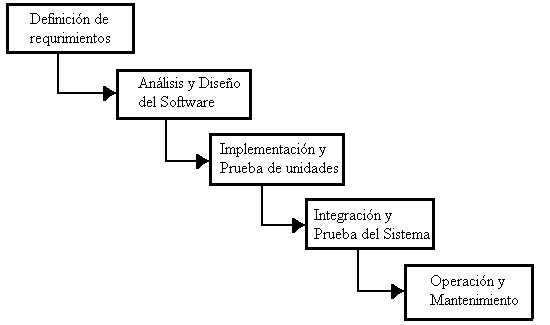
\includegraphics[scale=0.45]{M3_Modelo_Cascada}
	\caption{Modelo de proceso en cascada \cite{noauthor_archivo:modelo_nodate}}
	\label{fig:M3_Modelo_Cascada}
\end{figure}
\FloatBarrier

\begin{figure}[!h]
	\centering
	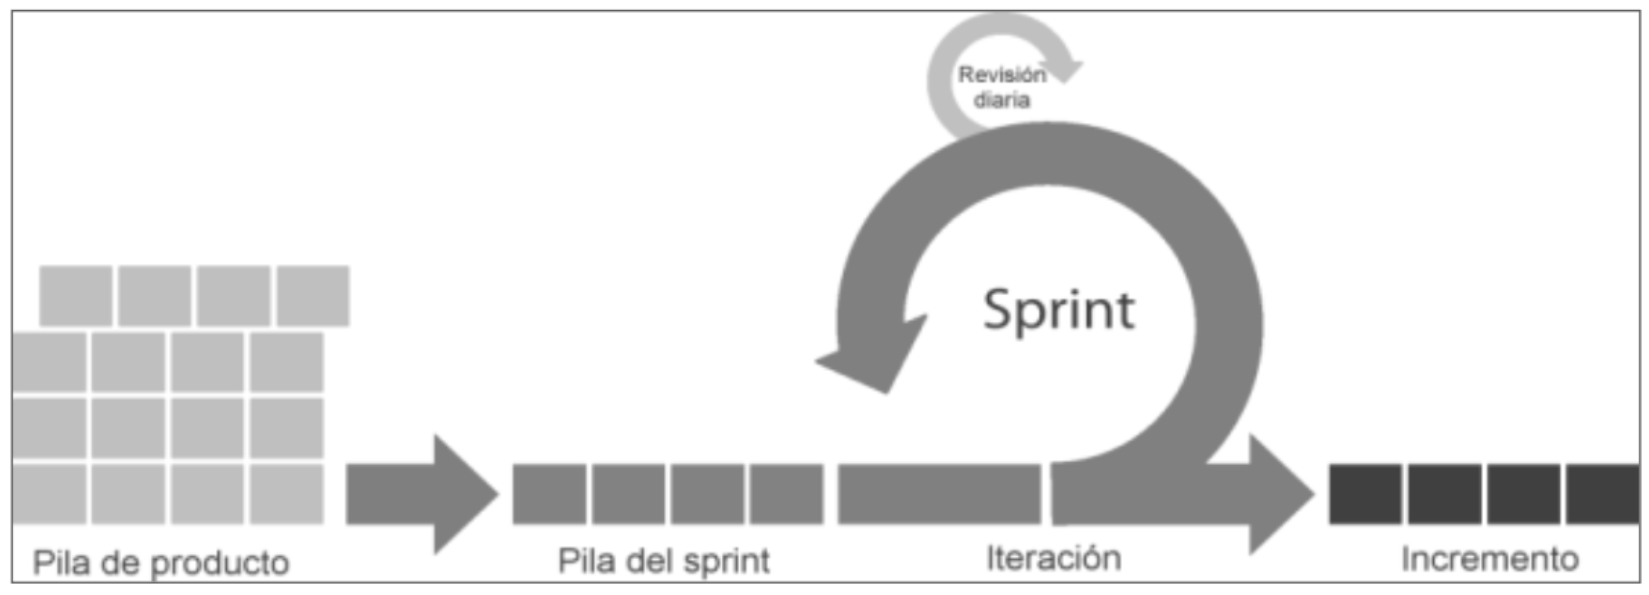
\includegraphics[scale=0.51]{M3_Scrum}
	\caption{Modelo de proceso incremental: Scrum \cite{noauthor_scrum_2019}}
	\label{fig:M3_Scrum}
\end{figure}
\FloatBarrier

Sin embargo, estos modelos generales deben ser extendidos y adaptados para crear modelos más específicos. No existe un único proceso ideal para construir todos los productos software, ya que este proceso depende de la naturaleza del proyecto y de otros factores como el equipo de desarrollo, la estabilidad de los requisitos funcionales, la importancia de los requisitos no funcionales como escalabilidad, seguridad, licencias, lenguaje de programación, tipo de arquitectura de computación, etc. Todos estos factores hacen que el proceso sea bastante complejo y que se requiera un modelo diferente para cada proyecto.

\section{Repositorios y forjas de proyectos software}

%\todo Este párrafo está repetido en la introducción. Pero tiene que ser reducido, en este apartado se puede detallar más extensamente con alguna captura de pantalla  que ayude a describir las equivalentes en múltiples repositorios.
%\todo revisar

En el apartado anterior se habla sobre la complejidad de un proceso software y que este puede ser representado por modelos que ayudan a organizar las diferentes actividades. En este apartado se hablará sobre metodologías y herramientas que pueden ayudar en más de una actividad del ciclo de vida.

Los repositorios de código son espacios virtuales donde los equipos de desarrollo generan los artefactos colaborativos procedentes de las actividades de un proceso de desarrollo. Estas herramientas permiten a un equipo de desarrollo trabajar en paralelo, lo que en ingeniería del software es complicado ya que , por lo general, miembros del mismo equipo necesitan trabajar sobre el mismo fichero y esto genera conflictos. Normalmente estos espacios se encuentran en servidores por motivos de seguridad y facilitar a los miembros del equipo puedan acceder al repositorio.

Un buen repositorio no solo permite almacenar los artefactos generados por cada una de las actividades del ciclo de vida del software. Sino que, también, permite llevar un historial de cambios e incluso ayudará a entender el contexto de la aplicación: quién ha realizado los cambios y porqué, es decir que permite almacenar las interacciones entre los miembros del equipo. Para ello se utilizan distintos sistemas, dependiendo del artefacto generado: foros de comunicación, sistemas de control de versiones como \textit{Git}, sistemas de gestión de incidencias, sistemas de gestión de pruebas, sistemas de revisiones de calidad, sistemas de integración y despliegue continuo, etc. \cite{guemes-pena_emerging_2018}.

Además de estos repositorios han surgido en la última década forjas de proyectos software de fácil acceso tanto para proyectos empresariales como para proyectos open-source (SourceForge \footnote{\url{https://sourceforge.net/}}, GitHub \footnote{\url{https://github.com/}}, GitLab \footnote{\url{https://about.gitlab.com/}}, Bitbucket  \footnote{\url{https://bitbucket.org/}}). Este mismo proyecto está almacenado en un repositorio en GitLab\footnote{Enlace al repositorio del proyecto en GitLab: \url{https://gitlab.com/mlb0029/comparador-de-metricas-de-evolucion-en-repositorios-software}}, ver Fig. \ref{fig:M3_ProyectoGitLab}.

\imagen{M3_ProyectoGitLab}{Captura de este proyecto almacenado en GitLab}

Estas forjas suelen ofrecer servidores para almacenar repositorios e integran múltiples sistemas para dar soporte a los flujos de trabajo y registrar las interacciones entre los miembros del equipo, también ofrecen posibilidades para usar estos sistemas en un servidor particular. Además dan la posibilidad de extensión funcional con sistemas de terceros para gestionar otras actividades no soportadas directamente por la propia forja, como Travis CI \footnote{\url{https://travis-ci.org/}} para gestionar la integración continua o Codacy \footnote{\url{https://www.codacy.com/}} para gestionar las revisiones automáticas de calidad como se puede observar en la Fig. \ref{fig:M3_Codacy}. 

\imagen{M3_Codacy}{Revisión automática de calidad realizada con Codacy sobre este proyecto}

Actualmente estas forjas han tenido una gran aceptación entre la comunidad de desarrolladores y existen muchos desarrollos de software de tendencia que las utilizan. En la Fig. \ref{fig:M3-TrendForja} se aprecia como cambia la tendencia de utilización de dichas forjas en el tiempo. Actualmente la forja predominante es claramente GitHub pero se ve un incremento en el uso de GitLab.

\imagen{M3-TrendForja}{Comparativa de tendencia de búsqueda de Google desde 2004 con los términos de distintas forjas de proyectos software}

 Estas forjas de proyectos software están en constante evolución, tanto en sus estructuras estáticas como en sus interacciones dinámicas en los proyectos y se registran grandes conjuntos de datos difíciles de procesar. Sin embargo, las forjas de proyectos software proporcionan interfaces de programación específicas que permiten acceder a toda la información registrada.

El  desafío a la comunidad científica y empresarial  es constante mostrando un incremento en el interés en las aplicaciones de minería que mejoren sus sistemas de decisión \cite{guemes-pena_emerging_2018}. Estos datos que registran las forjas de repositorios pueden ser utilizados para mejorar estos sistemas de decisión en función de la evolución del proyecto.

\subsection{GitHub vs. GitLab}\label{sect:3_2_1_GitHubVSGitLab}

%\todo introducir la sección
%\todo Usa la información de esta página \url{https://about.gitlab.com/devops-tools/github-vs-gitlab.html} para recoger las características de los repositorios 
%y su comparación.

Se ha hablado anteriormente de las forjas de repositorios como GitHub o GitLab y se puede observar en la Fig. \ref{fig:M3-TrendForja} la tendencia en el uso de diferentes forjas. Se observa como GitHub predomina sobre las demás y como crece el uso de GitLab. En esta sección se comparan los aspectos más relevantes de estas dos tendencias según los servicios que ofrecen.

\subsubsection{CI/CD - Continuous Integration/Continuous Delivery}
La integración y despliegue continuo son prácticas sirve para para construir, probar y, en caso de tratarse de una página web o una aplicación web, desplegar la aplicación una vez se combinen los cambios en el repositorio central, como se puede observar en Fig. \ref{fig:M3_CI-CD}. Ambos ofrecen la posibilidad de realizar este proceso mediante software de terceros como \textit{Travis CI}. Sin embargo, GitLab ofrece ejecutores o \textit{runners} propios para llevar este proceso desde GitLab. De hecho, en este trabajo con repositorio en GitLab se ha realizado este proceso definiendo un flujo de trabajo de integración continua y despliegue continuo. Se detalla este flujo en en capítulo \ref{sect:5_4_1_CICD}.

\imagen{M3_CI-CD}{CI/CD con GitLab \cite{noauthor_gitlab_nodate}}

\subsubsection{Estadísticas e informes}
Ambos ofrecen estadísticas e informes sobre los datos que registran de los repositorios y pueden ser accedidos visualmente desde la web del repositorio o desde APIs de programación. Por ejemplo, las métricas que trabaja este proyecto se calculan a partir de datos proporcionados por estas APIs.

Algo que ofrece GitLab y no GitHub es la monitorización del rendimiento de las aplicaciones que se hayan desplegado.

\subsubsection{Importación y exportación de proyectos}
A diferencia de GitHub, GitLab ofrece la posibilidad de importar proyectos desde otras fuentes como GitHub, Bitbucket, Google Code, etc. También es posible exportar proyectos de GitLab a otros sistemas.

\subsubsection{Sistema de seguimiento de incidencias (issues)}
Ambos cuentan con un sistema de seguimiento de incidencias (\textit{issue tracking system} o \textit{issue tracker}), permiten crear plantillas para las incidencias, adornarlas con Markdown\footnote{Markdown es un lenguaje de marcado que facilita la aplicación de formato a un texto empleando una serie de caracteres de una forma especial\cite{lasso_que_2013}}, usar etiquetas o \textit{labels} para categorizarlas, asignarlas a uno o varios miembros del equipo y bloquearlas para que solo puedan comentarlas los miembros del equipo.

Sin embargo GitLab da un paso más y permite asignar peso a las tareas, crear \textit{milestones}, asignar fechas de vencimiento, marcar la incidencia como confidencial, relacionar incidencias, mover o copiar incidencias a otros proyectos, marcar incidencias duplicadas, exportarlas a CSV, entre otras cosas. Otros aspectos destacables de GitLab en cuanto a este tema son los gráficos Burndown de los milestones (ver Fig. \ref{fig:M3_BurndownChart}), acciones rápidas y la gestión de una lista de quehaceres (\textit{todos}) de un usuario cuándo a este se le asignan incidencias.

\imagen{M3_BurndownChart}{Ejemplo de gráfico burndown}

A diferencia de GitLab, GitHub mantiene un historial de cambios en los comentarios de una incidencia; permite asignar las incidencias a listas mediante ``drag and drop"; proporciona información útil al pasar el ratón por encima de elementos de la web como usuario, issues, etc.

\subsubsection{Wiki}
En ambas forjas es posible disponer de una wiki para el proyecto.

\subsubsection{Otros aspectos destacables}
\begin{itemize}
	\item GitHub permite repositorios 100\% binarios
	\item GitLab permite tener una instancia propia de GitLab en un servidor particular, lo que permite que se pueda gestionar software adicional dentro del servidor como sistemas de detección de intrusos o un monitor de rendimiento.
	\item GitLab permite elegir miembros del equipo como revisores de ``\textit{merge requests}''.
	\item El código de Gitlab EE puede ser modificado para ajustarlo a las necesidades de seguridad y desarrollo.
	\item Ambos incluyen APIs que permiten realizar aplicaciones que se integren con GitLab o GitHub. Esto ha sido clave para la realización de este proyecto, como se ha mencionado anteriormente.
	\item GitLab nos proporciona un  IDE\footnote{Integrated Development Environment - Entorno de Desarrollo Integrado } web para realizar modificaciones sobre el código desde el mismo GitLab, también incluye un terminal web para el IDE que permite, por ejemplo, compilar el código.
	\item Ambos permiten la integración con repositorios Maven\footnote{Software de gestión de proyectos software: \url{https://maven.apache.org/}}
\end{itemize}

\section{Calidad de un producto software}

El software debe tener la funcionalidad y el rendimiento requeridos por el usuario, además de ser mantenible, confiable, eficiente y fácil de utilizar.

La calidad de un producto de software no tiene que ver solo con que se cumplan todos los requisitos funcionales, sino también otros requerimientos no funcionales que no se incluyen en la especificación como los de mantenimiento, eficiencia y usabilidad.

%Comentar fig 25.3 - Ppales factores de la calidad de protducto software p561
Sommerville enumera en \textit{Software Engineering} \cite{sommerville_ingenierisoftware_2002} los principales factores que afectan a la calidad del producto, como se puede observar en la Fig. \ref{fig:M3-FactoresCalidad}:
\begin{itemize}
	\tightlist
	\item Calidad del proceso
	\item Tecnología de desarrollo
	\item Calidad del personal
	\item Costo, tiempo y duración
\end{itemize}
\begin{figure}[!h]
	\centering
	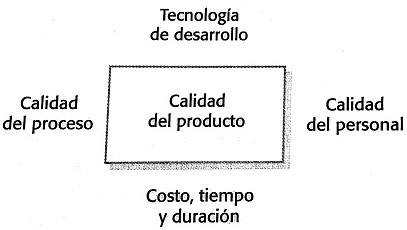
\includegraphics[scale=0.7]{M3-FactoresCalidad}
	\caption{Principales factores de calidad del producto de software\cite{sommerville_ingenierisoftware_2002}}\label{fig:M3-FactoresCalidad}
\end{figure}
\FloatBarrier

%Comentar fig 24.9 p549 relacion de metricas de proc y de prod

Para llegar a tener un software de calidad hay que tener en cuenta todos los factores mencionados anteriormente en cada una de las tres fases de la \textbf{administración de la calidad}: aseguramiento, planificación y control.

\begin{description}
	\item[Aseguramiento de la calidad.] Se encarga de establecer un marco de trabajo de procedimientos y estándares que guíen a construir software de calidad.
	\item[Planificación de la calidad.] Selección de procedimientos y estándares para un proyecto software especifico.
	\item[Control de la calidad.] La fase de control es la que se encarga de que el equipo de desarrollo cumpla los estándares y procedimientos definidos en el plan de calidad del proyecto. Esta fase puede realizarse mediante revisiones de calidad llevados a cabo por un grupo de personas y/o mediante un proceso automático llevado a cabo por algún programa.
\end{description}

%Comentar fg 24.1 p537 admin de calida en el proceso y desarrollo de software

\subsection{Control de la calidad: medición}

La fase de control de calidad es en la que se vigila que se sigan los procedimientos y estándares definidos en el plan de calidad. Pero estos podrían no ser adecuados o siempre pueden mejorar, por lo que en esta fase se puede valorar el mejorarlos como se puede observar en la Fig. \ref{fig:M3_CalidadProcesos}.

\imagen{M3_CalidadProcesos}{Calidad basada en procesos \cite{sommerville_ingenierisoftware_2002}}

Este proceso puede ser llevado a cabo mediante revisiones llevadas a cabo por un grupo de personas o por medio de programas que automaticen este proceso. El  desafío a la comunidad científica y empresarial es constante mostrando un incremento en el interés de aplicaciones que permiten  mejorar sus sistemas de decisión. Estas aplicaciones deberán llevar un control sobre el proceso y/o sobre el producto software y ese control se podrá realizar mediante un proceso de medición, esto ofrece una medida cuantitativa de los atributos del producto y del proceso software. 

La medición del software es un proceso en el cual se asignan valores numéricos o simbólicos a atributos de un producto o proceso software. Una métrica de software es una medida cuantitativa del grado en que un sistema, componente o proceso software posee un atributo dado. Las métricas son de control o de predicción. Las \textbf{métricas de control} se asocian al proceso de desarrollo del software, por ejemplo, la media de días que se tarda en cerrar una incidencia; y las \textbf{métricas de predicción} se asocian a productos software, por ejemplo, la complejidad ciclomática de una función. Y ambos tipos de métricas influyen en la toma de decisiones administrativas como se observa en la Fig. \ref{fig:M3-MetricasProcesoYProducto}. Los repositorios y las forjas facilitan la obtención de datos para este proceso de medición.

\imagen{M3-MetricasProcesoYProducto}{Métricas de control y métricas de predicción\cite{sommerville_ingenierisoftware_2002}}

Este proyecto se centra solo en la obtención de métricas de evolución que permitirán controlar y evaluar el proceso del desarrollo de un producto software. Por tanto se dejarán las métricas de predicción para otros trabajos y se detallará más sobre las de control en el siguiente apartado.

\subsection{Métricas de control: medición de la evolución o proceso de software}\label{sect:3_3_2_MetricasControl}

En la Fig. \ref{fig:M3-FactoresCalidad} se muestra la calidad de proceso como factor que afecta directamente a la calidad de producto. Parece lógico considerar como hipótesis que la calidad de un artefacto software tenga alguna relación con la manera en la que el equipo de desarrollo aplica las actividades del ciclo de vida del software dentro del repositorio. La validación empírica de estas  hipótesis ha abierto una nueva línea de aplicación con los conjuntos de datos que se pueden extraer de los repositorios gracias a interfaces de programación específicas que proporcionan estas forjas de repositorios y que permiten acceder a toda la información registrada.

Una plataforma de desarrollo colaborativo como GitLab puede presentar herramientas para controlar la evolución de un proyecto software. Por ejemplo un sistema de control de versiones (VCS - \textit{Version Control System}) como Git, un sistema de seguimiento de incidencias (\textit{Issue tracking system}), un sistema de integración continua (CI - \textit{Continuous Integration}), un sistema de despliegue continuo (CD - \textit{Continuous deploymen}t), etc.
Todas estas herramientas facilitan la comunicación entre los miembros de un equipo de desarrollo, ayudan a gestionar los cambios que producen cada uno de los miembros y proporcionan mediciones de proceso. Estas mediciones se pueden utilizar para obtener métricas de control que ayuden evaluar y mejorar la evolución del proyecto.

Las métricas de control que se utilizan en este proyecto provienen una Master Tesis titulada \textit{sPACE: Software Project Assessment in the Course of Evolution} \cite{ratzinger_space:_2007}. 
A continuación se describen las métricas que se implementan en este proyecto usando la plantilla de definición de la norma ISO 9126.

%\todo Cuando se ponen las fórmulas se puede utilizar el entorno matemático de Latex, mejora mucho la presentación.
%\todo Se puede utilizar el editor de Latex Web  \url{https://www.codecogs.com/latex/eqneditor.php?lang=es-es}
%\todo Un ejemplo de especificación  Sumatorio de (TCi-TCj) desde i=1, j=0 hasta i=NTC] / NTC. NTC
%\todo aplicando los entornos matemáticos $\frac{\sum_{i=1,j=0}^{NTC} TC_i - TC_j}{NTC}$
 
\textbf{\underline{I1 - Número total de issues (incidencias)}}

\begin{itemize}
	\item \textbf{Categoría}: Proceso de Orientación
	\item \textbf{Descripción}: Número total de issues creadas en el repositorio
	\item \textbf{Propósito}: ¿Cuántas issues se han definido en el repositorio?
	\item \textbf{Fórmula}: $NTI$. \textit{NTI = número total de issues}
	\item \textbf{Fuente de medición}: Proyecto en una plataforma de desarrollo colaborativo.
	\item \textbf{Interpretación}: $NTI \geq 0$. Valores bajos indican que no se utiliza un sistema de seguimiento de incidencias, podría ser porque el proyecto acaba de comenzar
	\item \textbf{Tipo de escala}: Absoluta
	\item \textbf{Tipo de medida}: \textit{NTI = Contador}
\end{itemize}

\textbf{\underline{I2 - Commits (cambios) por issue}}

\begin{itemize}
	\item \textbf{Categoría}: Proceso de Orientación
	\item \textbf{Descripción}: Número de commits por issue
	\item \textbf{Propósito}: ¿Cuál es el volumen medio de trabajo de las issues?
	\item \textbf{Fórmula}: $CI = \frac{NTC}{NTI}$. \textit{CI = Cambios por issue, NTC = Número total de commits, NTI = Numero total de issues}
	\item \textbf{Fuente de medición}: Proyecto en una plataforma de desarrollo colaborativo.
	\item \textbf{Interpretación}: $CI \geq 1$, Lo normal son valores altos. Si el valor es menor que uno significa que hay desarrollo sin documentar.
	\item \textbf{Tipo de escala}: Ratio 
	\item \textbf{Tipo de medida}: \textit{NTC, NTI = Contador}
\end{itemize}

\textbf{\underline{I3 - Porcentaje de issues cerradas}}

\begin{itemize}
	\item \textbf{Categoría}: Proceso de Orientación
	\item \textbf{Descripción}: Porcentaje de issues cerradas
	\item \textbf{Propósito}: ¿Qué porcentaje de issues definidas en el repositorio se han cerrado?
	\item \textbf{Fórmula}: $PIC = \frac{NTIC}{NTI}*100$. \textit{PIC = Porcentaje de issues cerradas, NTIC = Número total de issues cerradas, NTI = Numero total de issues}
	\item \textbf{Fuente de medición}: Proyecto en una plataforma de desarrollo colaborativo.
	\item \textbf{Interpretación}: $0 \leq PIC \leq 100$. Cuanto más alto mejor
	\item \textbf{Tipo de escala}: Ratio
	\item \textbf{Tipo de medida}: \textit{NTI, NTIC = Contador}
\end{itemize}

\textbf{\underline{TI1 - Media de días en cerrar una issue}}

\begin{itemize}
	\item \textbf{Categoría}: Constantes de tiempo
	\item \textbf{Descripción}:  Media de días en cerrar una issue
	\item \textbf{Propósito}: ¿Cuánto se suele tardar en cerrar una issue? 
	\item \textbf{Fórmula}: $MDCI = \frac{\sum_{i=0}^{NTIC}DCI_i}{NTIC}$. \textit{MDCI = Media de días en cerrar una issue, NTIC = Número total de issues cerradas, DCI = Días en cerrar la issue}
	\item \textbf{Fuente de medición}: Proyecto en una plataforma de desarrollo colaborativo.
	\item \textbf{Interpretación}: $MDCI \geq 0$. Cuanto más pequeño mejor. Si se siguen metodologías ágiles de desarrollo iterativo e incremental como SCRUM, la métrica debería indicar la duración del \textit{sprint} definido en la fase de planificación del proyecto. En SCRUM se recomiendan duraciones del \textit{sprint} de entre una y seis semanas, siendo recomendable que no exceda de un mes\cite{noauthor_scrum_2019}.
	\item \textbf{Tipo de escala}: Ratio
	\item \textbf{Tipo de medida}: \textit{NTI, NTIC = Contador}
\end{itemize}

\textbf{\underline{TC1 - Media de días entre commits}}

\begin{itemize}
	\item \textbf{Categoría}: Constantes de tiempo
	\item \textbf{Descripción}: Media de días que pasan entre dos commits consecutivos
	\item \textbf{Propósito}: ¿Cuántos días suelen pasar desde un commit hasta el siguiente?
	\item \textbf{Fórmula}: $MDC = \frac{\sum_{i=1}^{NTC} TC_i - TC_{i-1}}{NTC}$. $TC_i - TC_{i-1}$ en días; \textit{MDC = Media de días entre cambios, NTC = Número total de commits, TC = Tiempo de commit}
	%$MDEC = [Sumatorio de (TCi-TCj) desde i=1, j=0 hasta i=NTC] / NTC. NTC = Número total de commits, TC = Tiempo de Commit$ 
	\item \textbf{Fuente de medición}: Proyecto en una plataforma de desarrollo colaborativo.
	\item \textbf{Interpretación}: $MDEC \geq 0$. Cuanto más pequeño mejor. Se recomienda no superar los 5 días.
	\item \textbf{Tipo de escala}: Ratio
	\item \textbf{Tipo de medida}: \textit{NTC = Contador; TC = Tiempo}
\end{itemize}

\textbf{\underline{TC2 - Días entre primer y último commit}}

\begin{itemize}
	\item \textbf{Categoría}: Constantes de tiempo
	\item \textbf{Descripción}: Días transcurridos entre el primer y el ultimo commit 
	\item \textbf{Propósito}: ¿Cuantos días han pasado entre el primer y el último commit?
	\item \textbf{Fórmula}: $DEPUC = TC2- TC1$. $TC2- TC1$ en días;  \textit{DEPUC = Días entre primer y último commit, TC2 = Tiempo de último commit, TC1 = Tiempo de primer commit}
	\item \textbf{Fuente de medición}: Proyecto en una plataforma de desarrollo colaborativo.
	\item \textbf{Interpretación}: $DEPUC \geq 0$. Cuanto más alto, más tiempo lleva en desarrollo el proyecto. En procesos software empresariales se debería comparar con la estimación temporal de la fase de planificación. 
	\item \textbf{Tipo de escala}: Absoluta
	\item \textbf{Tipo de medida}: \textit{TC = Tiempo}
\end{itemize}

\textbf{\underline{TC3 - Ratio de actividad de commits por mes}}

\begin{itemize}
	\item \textbf{Categoría}: Constantes de tiempo
	\item \textbf{Descripción}: Muestra el número de commits relativos al número de meses
	\item \textbf{Propósito}:¿Cuál es el número medio de cambios por mes?
	\item \textbf{Fórmula}: $RCM = \frac{NTC}{NM}$. \textit{RCM = Ratio de cambios por mes, NTC = Número total de commits, NM = Número de meses que han pasado durante el desarrollo de la aplicación}
	\item \textbf{Fuente de medición}: Proyecto en una plataforma de desarrollo colaborativo.
	\item \textbf{Interpretación}: $RCM > 0$. Cuanto más alto mejor
	\item \textbf{Tipo de escala}: Ratio
	\item \textbf{Tipo de medida}: \textit{NTC = Contador}
\end{itemize}

\textbf{\underline{C1 - Cambios pico}}

\begin{itemize}
	\item \textbf{Categoría}: Constantes de tiempo
	\item \textbf{Descripción}: Número de commits en el mes que más commits se han realizado en relación con el número total de commits
	\item \textbf{Propósito}: ¿Cuál es la proporción de trabajo realizado en el mes con mayor número de cambios?
	\item \textbf{Fórmula}: $CP = \frac{NCMP}{NTC}$. \textit{CP = Cambios pico, NCMP = Número de commits en el mes pico, NTC = Número total de commits}
	\item \textbf{Fuente de medición}: Proyecto en una plataforma de desarrollo colaborativo.
	\item \textbf{Interpretación}: $0 \leq CCP \leq 1$. Mejor valores intermedios. Se recomienda no superar el 40\% del trabajo en un mes.
	\item \textbf{Tipo de escala}: Ratio
	\item \textbf{Tipo de medida}: \textit{NCMP, NTC = Contador}
\end{itemize}

\subsection{Framework de medición}\label{sect:3_3_3_FrameworkMedicion}

Para la implementación de las métricas se ha seguido la solución basada en frameworks propuesta en \textit{Soporte de Métricas con Independencia del Lenguaje para la Inferencia de Refactorizaciones} \cite{marticorena_soporte_2005}. El objetivo del \textit{framework} es la reutilización en la implementación del cálculo de métricas. Este diseño, mostrado en la Fig. \ref{fig:MCTMotorMetricas}, permite:

\begin{itemize}
	\item Facilitar el desarrollo de nuevas métricas
	\item Personalizar de los valores límite inferior y superior ya que estos pueden variar dependiendo del contexto en el que se calculen las métricas.
	\item Crear un grupo de configuraciones de métricas, de forma que se podrían calcular todas las métricas de ese grupo y almacenar los resultados en un colector de tipo \textit{MetricResult}
\end{itemize}

%Describir el diseño del motor de métricas, nombrar puntos de extensión
\imagen{MCTMotorMetricas}{Diagrama del framework para el cálculo de métricas con perfiles que almacena valores umbrales.}

En el diagrama UML de la Fig. \ref{fig:MCTMotorMetricas} se muestran las entidades principales del framework de medición y la relación entre ellas, especificando la navegabilidad y la multiplicidad. Las anotaciones en forma de flecha oscura especifican los patrones de diseño\citep{gamma_patrones_2002} aplicados en el framework.

Para crear una nueva métrica, esta deberá extender de la clase abstracta \textit{Metric} e implementar los métodos \textit{check()} y \textit{run()}. El método \textit{calculate()} de la clase \textit{Metric} utiliza el patrón de diseño \textbf{método plantilla}\footnote{\url{https://refactoring.guru/design-patterns/template-method}} que utiliza estos dos métodos, que deberán ser implementados por las clases concretas que hereden de \textit{Metric}. Un ejemplo de este método sería:

\begin{minipage}{\linewidth}
{\tiny
\begin{lstlisting}[breaklines]
...
Value calculate(Entity entity, 
		MetricConfiguration metricConfig, 
		MetricsResults metricsResults) 
{
  Value value;
  if(check(entity))
  {
    value = run(entity);
    metricsResults.addMeasure(new Measure(metricConfig, value));
  }
  return value;
}
...
\end{lstlisting}
}
\end{minipage}

Siendo \textit{entity} la entidad que se está midiendo, \textit{metricConfig} la configuración de valores limite que se está utilizando, \textit{metricsResults} el lugar donde se almacena el resultado y \textit{value} el valor medido en el método \textit{run()}. La plantilla establece que primero se comprueba que se pueda calcular la métrica y en ese caso se calcula y se añade a la coleción \textit{metricsResults}. 
Este método delega en las subclases el comportamiento de los métodos \textit{check()} y \textit{run()}. Además, almacena en el objeto colector \textit{metricsResults}, pasado como argumento, el valor medido para la configuración de la métrica para posibilitar el análisis y presentación de los resultados posteriores.

\textit{MetricConfiguration} toma el rol de decorador en el patrón de diseño \textbf{decorador}\footnote{\url{https://refactoring.guru/design-patterns/decorator}} que permite configurar los valores límite de las métricas. Implementa la misma interfaz que \textit{Metric}, \textit{IMetric}, y esta asociado a una métrica. Su método \textit{calculate()} simplemente llamará al método \textit{calculate()} de la métrica (\textit{Metric}) a la que esta asociada la configuración.

Un perfil de métricas agrupa un conjunto de configuraciones de métricas para un contexto dado, por ejemplo, para un conjunto de proyectos realizados por alumnos de la universidad en su realización del TFG. Se podría instanciar un \textit{MetricResult} para almacenar los resultados de toda esta colección de configuraciones de métricas y bastaría solo con recorrer el perfil usando el método \textit{calculate()} de cada configuración.

Este TFG ha adaptado este framework en el paquete ``motor de métricas'', y se han realizado unas pocas modificaciones. Las modificaciones más destacadas son:

\begin{itemize}
	\tightlist
	\item Se ha aplicado a las métricas concretas el patrón \textit{\textbf{Singleton}}\footnote{\url{https://refactoring.guru/design-patterns/singleton}}, que obliga a que solo haya una única instancia de cada métrica; y se ha aplicado el patrón \textit{\textbf{Método fábrica}}\footnote{\url{https://refactoring.guru/design-patterns/factory-method}} tal y como se muestra en la Fig. \ref{fig:M3_CambiosFrameworkMedicion1}, de forma que \textit{MetricConfiguration} no este asociada con la métrica en si, sino con una forma de obtenerla.\\
	La intencionalidad de esto es facilitar la persistencia de un perfil de métricas. Las métricas, se podrían ver como clases estáticas, no varían en tiempo de ejecución y solo debería haber una instancia de cada una de ellas. Por ello, al importar o exportar un perfil de métricas con su conjunto de configuraciones de métricas, estas configuraciones no deberían asociarse a la métrica, sino a la forma de acceder a la única instancia de esa métrica. 
	\item Se han añadido los métodos \textit{evaluate()} y \textit{getEvaluationFunction()} en la interfaz \textit{IMetric}, ver Fig. \ref{fig:M3_CambiosFrameworkMedicion2}.\\
	Esto permitirá interpretar y evaluar los valores medidos sobre los valores límite de la métrica o configuración de métrica. Por ejemplo, puede que para unas métricas un valor aceptable esté comprendido entre en valor límite superior y el valor límite inferior; y para oras un valor aceptable es aquel que supere el límite inferior.\\
	\textit{EvaluationFunction} es una interfaz funcional\footnote{
		\begin{itemize}
			\tightlist
			\item \url{https://docs.oracle.com/javase/8/docs/api/java/lang/FunctionalInterface.html}
			\item \url{https://docs.oracle.com/javase/8/docs/api/java/util/function/package-summary.html}
		\end{itemize}} 
	de tipo \textit{función}, recibe uno o más parámetros y devuelve un resultado. Este tipo de interfaces son posibles a partir de la versión 1.8 de Java \cite{noauthor_functionalinterface_nodate}.\\
	Esto permite definir los tipos de los parámetros y de retorno de una función que se puede almacenar en una variable. De esta forma se puede almacenar en una variable la forma en la que se puede evaluar la métrica.
\end{itemize}

\imagen{M3_CambiosFrameworkMedicion1}{Patrones ``singleton'' y ``método fábrica'' sobre el framework de medición}

\imagen{M3_CambiosFrameworkMedicion2}{Añadido al framework de medición la evaluación de métricas}
\capitulo{4}{Técnicas y herramientas}

%Esta parte de la memoria tiene como objetivo presentar las técnicas metodológicas y las herramientas de desarrollo que se han utilizado para llevar a cabo el proyecto. Si se han estudiado diferentes alternativas de metodologías, herramientas, bibliotecas se puede hacer un resumen de los aspectos más destacados de cada alternativa, incluyendo comparativas entre las distintas opciones y una justificación de las elecciones realizadas. 
%No se pretende que este apartado se convierta en un capítulo de un libro dedicado a cada una de las alternativas, sino comentar los aspectos más destacados de cada opción, con un repaso somero a los fundamentos esenciales y referencias bibliográficas para que el lector pueda ampliar su conocimiento sobre el tema.
Este capitulo muestra las técnicas y herramientas que se han utilizado para la alcanzar los objetivos del proyecto. 

\section{Herramientas utilizadas}

En este apartado se enumerarán las herramientas y una breve descripción del uso de las mismas, junto con alguna captura de pantalla. Sin embargo, hay explicaciones más detalladas sobre el código y otros aspectos relevantes sobre estas herramientas en el `Apéndice D - Documentación técnica de programación'.

\subsection{Entorno de desarrollo}
%\todo En todas las herramientas describir brevemente las funcionalidades de que se utilizan concretamente en el proyecto.
%\todo Se pueden acompañar con alguna captura de pantalla, porción de código y a una referencia al manual del progromador para obtener más detalle.
%\todo Por ejemplo Java SE v11.0.1 Expresiones Lambda en el uso de stream. 
% \todo Apache Maven indicar brevemente el  flujo de trabajo utilizado de compilación, testing, calidad, package y despliegue 
El entorno de desarrollo es el conjunto de herramientas que se utilizan para facilitar el desarrollo del software.

\begin{description}
	\item[Eclipse IDE for Java EE Developers.] Entorno de programación Java para aplicaciones web. 
	
		Se ha utilizado la versión: 2018-09 (4.9.0). Enlace a página de descarga:
		
		\url{https://www.eclipse.org/downloads/}
	
		Eclipse es de los entornos de programación más conocidos del mundo Java, aunque también hay paquetes de eclipse que dan soporte a otros lenguajes y sistemas. 
		
		\textit{Eclipse IDE for Java EE Developers} provee de un amplio conjunto de herramientas para facilitar el desarrollo de proyectos software Java y aplicaciones web. Es una versión más completa que \textit{Eclipse IDE for Java Developers}. Incluye un Java IDE (Java Integrated Development Environment - Entorno de Desarrollo Integrado), y herramientas para trabajar con Maven, Git y otras tecnologías. 
		
		Además es posible instalar plugins para ampliar las herramientas de desarrollo. Se han instalado varios de estos plugins como \textit{YEdit} para facilitar el trabajo con ficheros con un formato especial. Por ejemplo, \textit{YEdit} sirve como editor de ficheros con extensión \textit{.yml}, y ha sido utilizado para generar el fichero que configura la integración y despliegue continuo en GitLab. No tienen especial trascendencia y han sido descargados mediante sugerencias de Eclipse al abrir el fichero por primera vez. El plugin más importante que se ha instalado es \textit{Vaadin Plugin for Eclipse 4.0.2} que facilita el uso de la herramienta Vaadin en el entorno de Eclipse.
		
		Eclipse dispone de varias perspectivas dependiendo del trabajo que se quiera realizar en el proyecto, las que más se han utilizado son:
		\begin{itemize}
			\item \textbf{Java EE}. Es la perspectiva por defecto de este paquete de Eclipse, facilita el trabajo de aplicaciones web. Es la perspectiva que se ha utilizado para escribir código. Ofrece, entre otras cosas, un explorador de paquetes y vistas para trabajar con Java.
			\item \textbf{Debug}. La perspectiva que se utiliza para depurar el programa. Sirve para ejecutar la aplicación instrucción a instrucción y detectar así un problema o \textit{bug}.
			\item \textbf{Git}. Esta perspectiva permite trabajar con el sistema de control de versiones Git. Mantiene una vista con un listado de repositorios, otra que visualiza el historial de cambios de un archivo seleccionado y, la más importante, una ventana de que permite visualizar los cambios realizados, indexarlos, realizar commits y publicarlos en el repositorio remoto. Eclipse permite la integración con GitLab y cualquier otra forja de repositorios.
		\end{itemize}
		
	\item[Java SE 11 (JDK).] \textit{Java Development Kit}. Conjunto de herramientas software útiles para el desarrollo de aplicaciones en Java entre las que se incluyen \textit{javac.exe}, el compilador de Java; \textit{javadoc.exe}, para generar documentación; y \textit{java.exe}, el intérprete de Java.
	
		Se ha utilizado la versión  v11.0.1. Enlace a página de descarga:
		
		\url{https://www.oracle.com/technetwork/java/javase/downloads/index.html}
	
		Se ha utilizado la última versión de Java al comenzar el desarrollo, actualmente ha sido lanzada la versión \textit{Java SE 12.0.2} y se esperan actualizaciones cada 6 meses. Sin embargo, ha sido posible compilar y ejecutar tanto las pruebas como la aplicación web con Java 8 realizando dos pequeñas modificaciones:
		\begin{itemize}
			\item De la versión 11 se ha utilizado el método \textit{isBlank()} de la clase \textit{String}. Se diferencia de \textit{isEmpty()} en que no comprueba la longitud de la cadena y devuelve \textit{true} si es 0, sino que devuelve \textit{true} si la longitud es 0 o si no es 0 pero todos los caracteres de la cadena son espacios en blanco.
			\item De la clase \textit{java.util.Optional} \footnote{\url{https://docs.oracle.com/en/java/javase/11/docs/api/java.base/java/util/Optional.html}}, soportada desde la versión 1.8, se utiliza la función \textit{orElseThrow()}, que se soporta desde la versión 10, por tanto habría que buscar una alternativa para pasar a la versión 1.8. La versión 11 trae a esta clase la función \textit{isEmpty()}.
		\end{itemize}
	\item[Apache Maven.] Gestor de proyectos software que ayuda en la construcción del proyecto, la generación de documentación, generación de informes, gestión de dependencias, integración con un sistema de control de versiones, etc. 
	
		Se ha utilizado la versión  v3.6.0. Enlace a página de descarga:
		
		\url{https://maven.apache.org/download.cgi}
		
		Se han automatizado gracias a Maven y la integración continua (CI) de GitLab los siguientes procesos:
		\begin{itemize}
			\item Compilación. Es un proceso de generación de binarios a partir del código fuente escrito en Java.
			\item Pruebas unitarias y de integración automáticas con JUnit.
			\item Generación de informes de pruebas, cobertura y análisis de calidad con ayuda de Jacoco, JUnit y Codacy.
			\item Despliegue en servidor de Heroku.
		\end{itemize}
	
	\item[Apache Tomcat.] Contenedor de aplicaciones web con soporte de servlets Java. Sirve para desplegar la aplicación.
	
		Se ha utilizado la versión  v9.0.13. Enlace a página de descarga:
		
		\url{https://tomcat.apache.org/download-90.cgi}
		
		Se ha utilizado para desplegar en el equipo (computador) local de desarrollo y realizar pruebas manuales de despliegue, y de interfaz (Ver Fig. \ref{fig:M4_TomcatAppManager}). Es posible su integración con Eclipse.
		
		\begin{figure}[!h]
			\centering
			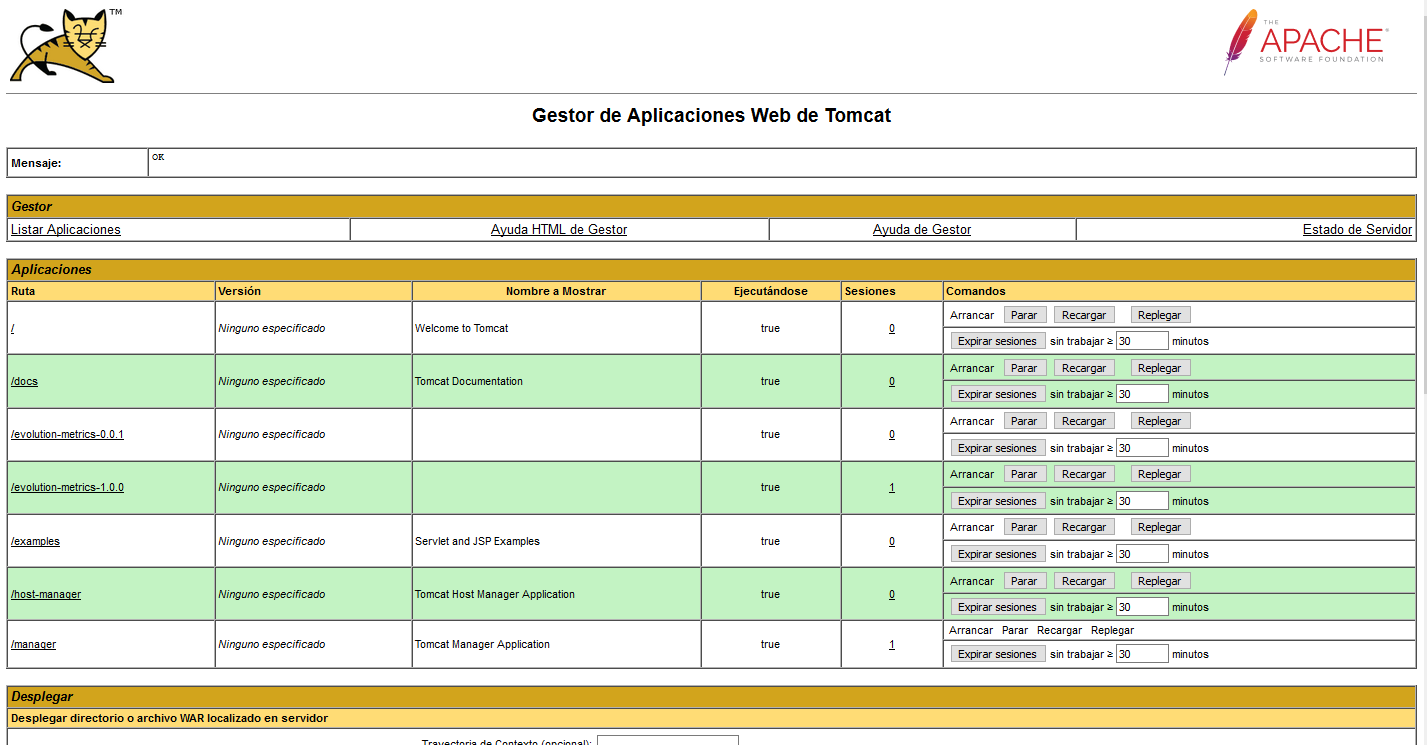
\includegraphics[scale=0.35]{M4_TomcatAppManager}
			\caption{Gestor de aplicaciones Tomcat con dos versiones desplegadas de la aplicación de este proyecto}\label{fig:M4_TomcatAppManager}
		\end{figure}
		\FloatBarrier
		
\end{description}
\subsection{Logging}
El proceso de logging permite registrar lo que ocurre dentro de la aplicación para poder identificar futuros problemas en tiempo de ejecución. Esto es especialmente útil en la fase de producción, después de haber desplegado la aplicación.
\begin{description}
	\item[SLF4J.] Fachada de logging.
	
		Enlace a página de descarga:
	
		\url{https://www.slf4j.org/download.html}
	
	\item[Log4j 2.] Logger. Se ha utilizado la versión  v2.11.2.
	
	 	Enlace a página de descarga:
	
	 	\url{https://logging.apache.org/log4j/2.x/download.html}
	
		SLF4J (\textit{Simple Logging Facade for Java}) es una capa intermedia entre el framework de logging como \textit{java.util.logging}, \textit{logback}, \textit{log4j}) y la aplicación, esto permite poder cambiar de framework de logging facilmente en tiempo de despliegue.
		
		Se utilizó Log4j al tener experiencia previa con esta herramienta. Esta herramienta permite configurar este proceso por medio de un fichero log4j2 con extensión XML, JSON, YAML o Properties\footnote{Manual de configuración de Log4j 2: \url{https://logging.apache.org/log4j/2.x/manual/configuration.html}} \citep{noauthor_log4j_nodate}. En este proyecto se configuró mediante un fichero con extensión \textit{.properties}. 
		
		Ambas herramientas están integradas con Maven, y solo es necesario añadir en el fichero \textit{pom.xml} las dependencias correspondientes.
	
\end{description}
\subsection{Pruebas}
La fase de pruebas permite probar que la implementación que se ha estado llevando a cabo funciona correctamente. Se han realizado dos tipos de pruebas: unitarias y de integración. Las unitarias prueban los diferentes módulos y las de integración prueban la relación que tienen los diferentes módulos entre sí.
\begin{description}
	\item[JUnit5]. Conjunto de bibliotecas para el desarrollo de pruebas unitarias. 
	
		Se ha utilizado la versión  v5.3.1. Enlace a página de descarga:
		
		\url{https://junit.org/junit5/}
		
		JUnit es una herramienta que se utiliza para realizar pruebas unitarias de forma automática o semiautomática de aplicaciones Java. Se han ejecutado de ambas formas. La automatización completa ha sido posible gracias a las herramientas de CI (\textit{Continuous Integration}) de GitLab.
		Esta versión de JUnit 5, sobre la anterior JUnit 4, ha influido en este proyecto de la siguiente manera:
		\begin{itemize}
			\item JUnit 5 soporta \textbf{Java 11}.
			
			\item Permite realizar asertos (\textit{asserts}) de tipo \textit{\textbf{assertAll()}} \footnote{\url{https://junit.org/junit5/docs/current/api/org/junit/jupiter/api/Assertions.html}}. Se realizó en pruebas en versiones previas pero luego se optó por quitarlos y utilizar asertos simples.
			
			\item Permite realizar \textbf{comprobaciones de lanzamiento de excepciones} en asertos del tipo \textit{assertThrows()}.
			
			\item Permite realizar presunciones (\textit{\textbf{assumptions}}) que permiten realizar una comprobación que pasará por alto el test (lo marca como \textit{skipped}) si la comprobación falla. Es decir que no lo marcará como error, simplemente no realizará el test. \\Esto ha sido útil de cara a probar funciones que realicen conexiones a GitLab que requieran credenciales de acceso. No es correcto publicar en los test las credenciales de acceso del programador a GitLab. Por tanto estos test tienen presunciones que comprueban que se tiene las credenciales de acceso y no se realizan los test si no se dispone de estas credenciales, en lugar de lanzar un error por no poder realizar la conexión. Por tanto estos test se ejecutan manualmente por el programador en su equipo local y no se ejecutan automáticamente en el proceso de integración continua de GitLab.
			
			\item Permite crear \textbf{test parametrizados}. Estos son test que prueban funciones que requieren argumentos. Cada combinación de argumentos es un caso de prueba y crear un test para cada combinación es un caso claro del defecto de código: `código duplicado'. Por ello estos argumentos se pueden generar mediante funciones, enumeraciones, proveedores de argumentos o recolectar desde un CSV y solo ser necesario un test para todas las combinaciones de argumentos posibles.
		\end{itemize}
\end{description}
\subsection{Frameworks y librerías específicas para el proyecto}
%\todo Además de los enlaces de la aplicación añade los enlaces de tu repositorio
\begin{description}
	\item[gitlab4j-api]. Framework de conexión a GitLab API. 
	
		Se ha utilizado la versión  v4.9.14. Enlace:
		
		\url{https://github.com/gitlab4j/gitlab4j-api}
		
		Se ha preferido frente a \textit{timols/java-gitlab-api} \footnote{\url{https://github.com/timols/java-gitlab-api}} tras realizar un estudio sobre sus métricas de evolución y una comparativa sobre la documentación. Concluyendo en que \textbf{gitlab4j-api} contiene mejor documentación, mejor evolución y, a día de hoy, sigue evolucionando.
		
	\item[Apache Commons Math]. Librería que se utiliza para matemáticas descriptivas utilizada para el cálculo de cuartiles para obtener los valores umbrales de las métricas según las estadísticas. 
	
		Se ha utilizado la versión  v3.6.1. Enlace a página de descarga:
	
		\url{https://commons.apache.org/proper/commons-math/download_math.cgi}
		
		Ejemplo de uso de la clase \textit{DescriptiveStatistics} de la librería:
		
\begin{minipage}{\linewidth}
{\tiny 
\begin{lstlisting}[breaklines]
...
ArrayList<Double> datasetForMetric;
Double q1ForMetric, q3ForMetric;
DescriptiveStatistics descriptiveStatisticsForMetric;

descriptiveStatisticsForMetric = new DescriptiveStatistics(datasetForMetric
	  .stream()
	  .mapToDouble(x -> x)
	  .toArray());
q1ForMetric = descriptiveStatisticsForMetric.getPercentile(25);
q3ForMetric = descriptiveStatisticsForMetric.getPercentile(75);
...
\end{lstlisting}
}
\end{minipage}		

\end{description}
\subsection{Interfaz gráfica}
\begin{description}
	\item[Vaadin]. Framework para desarrollo de interfaces Web con Java.
		Se ha utilizado la versión  v13.0.0 Enlace:
		
		\url{https://vaadin.com/}
		
		Con este framework no ha sido necesario escribir HTML, solo Java y un poco de CSS. Por ejemplo, para implementar un \textit{checkbox} se utilizaría el siguiente código:
		
\begin{minipage}{\linewidth}
{\tiny \begin{lstlisting}
...
Checkbox checkbox = new Checkbox();
checkbox.setLabel("Default Checkbox");
...
\end{lstlisting}}
\end{minipage}	
		y el resultado sería el de la Fig. \ref{fig:M4_Vaadin_ChkBox}
\begin{figure}[!h]
	\centering
	
\includegraphics[scale=0.5]{M4_Vaadin_ChkBox}
	\caption{Checkbox generado por Vaadin}\label{fig:M4_Vaadin_ChkBox}
\end{figure}
\FloatBarrier

\end{description}
\subsection{CI/CD y revisión automática}
\begin{description}
	\item[GitLab]. Plataforma de desarrollo colaborativo y forja de repositorios en la que se ha almacenado el proyecto en un repositorio Git.
	
		Enlace a GitLab:
		
		\url{https://gitlab.com/users/sign_in}
		
		Enlace al repositorio del proyecto:
		
		\url{https://gitlab.com/mlb0029/comparador-de-metricas-de-evolucion-en-repositorios-software}
		
		Para más información hay una comparativa entre GitHub y GitLab en la sección \ref{sect:3_2_1_GitHubVSGitLab}.
		
	\item[Codacy]. Herramienta de generación automática de informes de calidad de código.
	
		 Enlace a Codacy:
		 
		 \url{https://www.codacy.com/}
		 
		 Enlace a proyecto en Codacy: 
		 
		 \url{https://app.codacy.com/manual/mlb0029/comparador-de-metricas-de-evolucion-en-repositorios-software/dashboard}
	
	\item[JaCoCo]. Librería para cobertura de código en Java utilizada para generar informes de cobertura. Estos informes se pueden mostrar en GitLab fácilmente publicando los informes con formato HTML. También se han enviado estos informes a Codacy para que controle la cobertura además de la calidad de código.
	
		Se ha utilizado la versión v0.8.3.
		
		Enlace:
		
		\url{https://www.eclemma.org/jacoco/}
		
		Enlace a informe de JaCoCo en HTML sobre la cobertura del proyecto:
		
		\url{https://mlb0029.gitlab.io/comparador-de-metricas-de-evolucion-en-repositorios-software/}
	
	\item[Heroku]. Herramienta para despliegue continuo (CD).
	
		Enlace a herramienta:
		
		\url{https://id.heroku.com/login}
		
		Enlace a aplicación desplegada:
		
		\url{https://evolution-metrics.herokuapp.com/}
	
\end{description}
\subsection{Documentación}
\begin{description}
	\item[LaTeX]. Sistema de composición de textos.
		Enlace a herramienta:
		
		\url{https://www.latex-project.org/}
		
	\item[TeXstudio]. Entorno de desarrollo de documentos LaTeX.
	
		Enlace a herramienta:
		
		\url{https://www.texstudio.org/}
	
	\item[Zotero]. Herramienta de gestión de fuentes bibliográficas.
		
		Enlace a herramienta:
		
		\url{https://www.zotero.org/}
	
\end{description}
\subsection{Técnicas}
\begin{itemize}
	\item A lo largo del proyecto se han utilizado numerosos patrones de diseño \citep{gamma_patrones_2002} como Singleton, Factory Method, Wrapper, Builder, Listener, etc. Se detallará más sobre esto en los apéndices.
	
	\item Para el motor de métricas se ha utilizado como base el framework propuesto en \textit{Soporte de Métricas con Independencia del Lenguaje para la Inferencia de Refactorizaciones} \citep{marticorena_soporte_2005}. Ver Fig. \ref{fig:MCTMotorMetricas} en la sección \ref{sect:3_3_3_FrameworkMedicion}.
	
	\item El ciclo de vida del software de este proyecto ha seguido un modelo de proceso iterativo e incremental: Scrum \citep{noauthor_scrum_2019}. Este proceso de detalla en el siguiente capítulo.
\end{itemize}

%herramientas codacy maven, gitlab, capturas, etc, cobertura, heroku, ci, pipeline, token...
\capitulo{5}{Aspectos relevantes del desarrollo del proyecto}

%Este apartado pretende recoger los aspectos más interesantes del desarrollo del proyecto, comentados por los autores del mismo.
%Debe incluir desde la exposición del ciclo de vida utilizado, hasta los detalles de mayor relevancia de las fases de análisis, diseño e implementación.
%Se busca que no sea una mera operación de copiar y pegar diagramas y extractos del código fuente, sino que realmente se justifiquen los caminos de solución que se han tomado, especialmente aquellos que no sean triviales.
%Puede ser el lugar más adecuado para documentar los aspectos más interesantes del diseño y de la implementación, con un mayor hincapié en aspectos tales como el tipo de arquitectura elegido, los índices de las tablas de la base de datos, normalización y desnormalización, distribución en ficheros3, reglas de negocio dentro de las bases de datos (EDVHV GH GDWRV DFWLYDV), aspectos de desarrollo relacionados con el WWW...
%Este apartado, debe convertirse en el resumen de la experiencia práctica del proyecto, y por sí mismo justifica que la memoria se convierta en un documento útil, fuente de referencia para los autores, los tutores y futuros alumnos.

%Despliegue continuo - direccion de app en heroku. Sistema gratuito sirve para validar, pero no para explotar
%Diseño extensible
%Framework vaadin
%No responsive

%Comparacion de tfgs en la ubu, captura dde pantalla con comparativa tfg
Este capítulo recoge los aspectos más relevantes del ciclo de vida del proyecto y justifica los caminos que se han tomado durante el desarrollo. Se menciona el motivo de elección del proyecto, el modelo de ciclo de vida utilizado, una breve explicación de los aspectos de configuración del proyecto y el flujo de trabajo.

\section{Motivación de la elección y relación con asignaturas}

La elección de este trabajo fue motivada por su relación con la asignatura de \textit{Desarrollo Avanzado de Sistemas Software}. En esta se enseña como desarrollar software de calidad mediante el proceso de \textit{Administración de la calidad}, en la cual una de las actividades es el control de calidad. Este control se puede llevar a cabo mediante un proceso de medición. 

En este proyecto se han elegido métricas ya definidas para llevar un control sobre el ciclo de vida de uno o varios proyectos. Esto permite comprender el proceso de desarrollo, evaluarlo respecto a lo que se había planeado, predecir si los planes van por buen camino e identificar los defectos y mejorar la calidad del proceso. Además, esto ha podido ser comprobado, puesto que las mediciones realizadas por el software creado en este proyecto han servido para comparar este proceso con procesos de otros trabajos de fin de grado para saber si la evolución del proyecto era la adecuada.

Este proyecto tiene más relación con la asignatura de \textit{Desarrollo Avanzado de Sistemas Software} pero también se han tomado referencias e ideas de las siguientes materias: 
\begin{itemize}
	\tightlist
	\item De \textit{Estadística} el cálculo de cuartiles para calcular los valores umbrales de las métricas.
	\item De las asignaturas de \textit{Ingeniería del Software} y \textit{Análisis y Diseño de Sistemas}, todo lo relacionado con el ciclo de vida del software, el análisis de los requisitos y el modelado del sistema (diagramas de clases, diagramas de casos de uso, etc).
	\item De \textit{Interacción Hombre/Máquina}  el diseño de la interfaz y las características que este debería alcanzar como usabilidad, la facilidad de aprendizaje, simplicidad, adaptabilidad, etc.
	\item De \textit{Gestión de Proyectos} mayoritariamente el modelo de ciclo de vida del software: Scrum.
	\item De \textit{Diseño y Mantenimiento del Software} el uso de patrones de diseño para mejorar la calidad de código y mantener los principios SOLID  \footnote{Single responsability, Open/Closed, Liskov substitution, Interface segregation, Dependency inversion} y de \textit{Desarrollo Avanzado de Sistemas Software} la naturaleza del trabajo, las revisiones automáticas de calidad de código por medio de métricas y la importancia de la refactorización al detectar defectos de diseño.
	\item \textit{Validación y Pruebas} en la construcción de la batería de pruebas.
	\item \textit{Sistemas Distribuidos} ha ayudado en el uso de Maven y en la construcción de una aplicación web.
	\item \textit{Metodología de la Programación} y \textit{Estructuras de Datos} han contribuido en cuanto a la construcción de una aplicación en un lenguaje Orientado a Objetos.
\end{itemize}

\section{Modelo de ciclo de vida}

Tras la elección del proyecto se acordó definir una evolución que siga las bases del modelo \textit{\textbf{Scrum}}. Tomando un proceso de desarrollo incremental con revisión de las iteraciones cada dos semanas, la duración de un sprint. Estas revisiones se realizan por medio de reuniones que constaban de dos partes:
\begin{description}
	\item [Revisión del sprint:] Se revisa el incremento generado como resultado del sprint, se describen los problemas que hubo durante su desarrollo y se plantean mejoras sobre el incremento (se puede modificar la pila del producto o \textit{product backlog} \footnote{Lista de requisitos de usuario que, a partir de la visión inicial del producto, crece y evoluciona durante el desarrollo \cite{noauthor_scrum_2019}}) y soluciones a estos problemas.
	\item [Planificación del siguiente sprint:] Se definen las tareas que se deben ejecutar durante el siguiente sprint. Estas tareas en \textit{Scrum} se recogen en la pila del sprint o \textit{sprint backlog}.
\end{description}

Según la naturaleza de los sprints, en el proceso del desarrollo se pueden diferenciar varias etapas:
\begin{itemize}
	\item  Una primera etapa de \textbf{investigación} de las herramientas que se utilizarán durante el proceso y de \textbf{configuración} del entorno de desarrollo.
	\item En la segunda etapa se aprecian tareas de \textbf{diseño e implementación} de la parte lógica de la aplicación. Se diseña el framework de conexión a forjas de repositorios, se implementa el framework descrito en \textit{Soporte de Métricas con Independencia del Lenguaje para la Inferencia de Refactorizaciones}  \cite{marticorena_soporte_2005} para el cálculo de métricas y se diseñan los modelos de datos que serán utilizados por la aplicación.
	\item Durante la segunda etapa se apreció que se debía facilitar el \textbf{flujo de trabajo}, la comunicación entre tutor y alumno y facilitar las reuniones de revisión y planificación del sprint. Esto duro un sprint y se realizaron tareas como:
		\begin{itemize}
			\item Configurar la gestión del proyecto con Maven \footnote{Gestor de proyectos software que ayuda en la construcción del proyecto, la generación de documentación, la generación de informes, la gestión de dependencias, la integración con un sistema de control de versiones, etc.}
			\item Configurar los procesos de integración y despliegue continuo (CI/CD) con GitLab. En estos procesos se realizan actividades automáticamente cada cierto tiempo o cada vez que se realice algún cambio. Ejemplos de estas actividades serían: construir software (\textit{build}), realizar pruebas y revisar su cobertura, desplegar la aplicación en caso de que se trate de una aplicación web, revisar la calidad, etc.
			\item Realizar pruebas unitarias con JUnit y automatizar su ejecución gracias a Maven y los \textit{pipelines} \footnote{Definen las actividades de los procesos de CI/CD y las fases y el entorno en las que se ejecutarán} de GitLab.
			\item Configurar revisiones automáticas de calidad y de cobertura de las pruebas gracias a Maven, Codacy, JaCoCo y GitLab.
			\item Configurar un entorno en Heroku donde poder desplegar la aplicación entre las actividades de CI/CD y así poder ser revisada por el tutor fácilmente.
			\item Configurar badges \footnote{Son placas que aportan información rápida sobre el estado del proyecto en ciertos aspectos como la cobertura, la calidad de código o el estado del proceso de CI/CD} para representar el estado del proyecto en cuanto a calidad de código, cobertura, despliegue y los trabajos de CI/CD.
		\end{itemize}
	\item Etapa  de diseño e implementación de la \textbf{interfaz gráfica} y \textbf{mejora de funcionalidades}. A menudo, estas mejoras precisaban de modificaciones en la parte lógica de la aplicación.
	\item Etapa de \textbf{documentación} en la que se escribe la memoria y los anexos. También se preparan videotutoriales y manuales de usuario.
\end{itemize}

Para más detalles se puede consultar el \textit{Anexo A - Plan de Proyecto Software}. En este se muestra más información sobre estos sprints y el ciclo de vida del proyecto.

\section{Gestión del proyecto}

En esta sección se exponen y se justifican las principales decisiones que se han tomado en cuanto a la configuración del proyecto.

\subsection{Aplicación web}

Para alcanzar los objetivos del proyecto se ha decidido implementar una aplicación web. La principal diferencia es que no se instala en un equipo local sino que se accede a la aplicación desde un navegador web, después de que esta haya sido desplegada en un servidor. Esto tiene varias ventajas: 
\begin{itemize}
	\tightlist
	\item El usuario no necesita instalar la aplicación y puede acceder a ella directamente desde el navegador, esto evita costes de tiempo y de recursos del computador.
	\item  Portabilidad. Es posible que una aplicación de escritorio no pueda ser instalada en ciertos computadores debido a los recursos de los que disponen, el sistema operativo u otros factores. Una aplicación web solo depende del navegador que tenga instalado el computador y, normalmente, puede tener varios instalados. Además, se ha comprobado la portabilidad de navegador y la aplicación funciona en los principales navegadores: Mozilla Firefox, Microsoft Edge, Internet Explorer, Google Chrome y Opera.
	\item Actualizaciones. Para actualizar una aplicación web, el usuario final no tiene que instalar la actualización. Sino que habrá un periodo de mantenimiento de aplicación, normalmente muy corto y fuera de horario de uso, en el que ningún usuario podrá acceder a la aplicación. Después de este periodo, todos los usuarios dispondrán de la actualización.
\end{itemize}

\subsection{Java 11}

El proyecto se iba a desarrollar en Java desde el principio, era uno de los requisitos no funcionales iniciales. La elección de la versión fue uno de los temas que se discutieron al inicio del proyecto. Java 8 era la versión más conocida y la más estable, pero recientemente había surgido la versión 11 de Java. 

Se escogió la versión 11, por ser la más reciente \footnote{Actualmente, la versión Java SE 12.0.2 es la más reciente}. Esto supuso un estudio de las versiones que se debían utilizar de las herramientas que requieren de Java, como Tomcat \footnote{Para desplegar aplicaciones con Java 11 se requiere de la versión 9.0.x de Tomcat} y algunas otras configuraciones. Por ejemplo, se tuvo que configurar el fichero pom.xml del proyecto para que Maven compile en la versión 11 de Java:

\begin{minipage}{\linewidth}
{\tiny
\begin{lstlisting}[breaklines]
...
<properties>
	<project.build.sourceEncoding>UTF-8</project.build.sourceEncoding>
	<project.reporting.outputEncoding>UTF-8</project.reporting.outputEncoding>
	<java.version>11</java.version>
</properties>
...
<build>
...
	<plugins>
		<plugin>
			<groupId>org.apache.maven.plugins</groupId>
			<artifactId>maven-compiler-plugin</artifactId>
			<configuration>
				<source>${java.version}</source>
				<target>${java.version}</target>
			</configuration>
			<version>3.8.0</version>
		</plugin>
		<plugin>
			<groupId>org.apache.maven.plugins</groupId>
			<artifactId>maven-war-plugin</artifactId>
			<version>3.2.2</version>
		</plugin>
		...
	</plugins>
	...
</build>
...
\end{lstlisting}
}
\end{minipage}

Y en Eclipse IDE habría que añadir manualmente el JRE desde la ventana Window/Preferences, como se muestra en la Fig. \ref{fig:M5_Eclipse_Java11}.

\imagen{M5_Eclipse_Java11}{Añadir Java 11 a Eclipse}

Sin embargo, tampoco se trabajó demasiado con las nuevas funcionalidades que trae Java 11, ya que ha sido posible compilar el artefacto final con Java 1.8 y solo han hecho falta dos pequeños cambios:
\begin{itemize}
	\item De la versión 11 se ha utilizado el método \textit{isBlank()} de la clase \textit{String} \footnote{\url{https://docs.oracle.com/en/java/javase/11/docs/api/java.base/java/lang/String.html}}. Se diferencia de \textit{isEmpty()} en que no comprueba la longitud de la cadena y devuelve \textit{true} si es 0. Sino que devuelve \textit{true} si la longitud es 0, o si no es 0 pero todos los caracteres de la cadena son espacios en blanco.
	\item De la clase \textit{java.util.Optional} \footnote{\url{https://docs.oracle.com/en/java/javase/11/docs/api/java.base/java/util/Optional.html}}, soportada desde la versión 1.8, se utiliza la función \textit{orElseThrow()}, que se soporta desde la versión 10, por tanto habría que buscar una alternativa para pasar a la versión 1.8. La versión 11 trae a esta clase la función \textit{isEmpty()}.
\end{itemize}

Para saber más sobre las novedades de Java 11 es recomendable leer `\textit{JDK 11 Release Notes}' \cite{noauthor_jdk_nodate}. También hay un artículo que explica las principales diferencias entre Java 8 y Java 11 llamado `\textit{De Java 8 a Java 11, ¿aún no te has migrado?}' \cite{hoyo_java_2019}.

\subsubsection{Trabajo con streams de Java}

Desde Java 1.8 se puede trabajar con Streams. En este proyecto se ha dado gran uso de ellos ya que facilitan enormemente procesar grandes colecciones de datos. Estos permiten \textbf{filtrar} datos de una colección mediante un predicado, \textbf{ordenar} los datos mediante un comparador, \textbf{mapear} o \textbf{reducir} los datos mediante alguna función y \textbf{almacenarlos} en algún tipo de colección mediante un colector. El mapeo asocia cada dato del stream con un nuevo elemento, por ejemplo, de cada número de una colección numérica obtenemos su potencia de dos. Y la reducción es obtener un único resultado a partir del conjunto de datos, por ejemplo, obtener el máximo o la suma de todos los datos de un conjunto numérico.

A continuación se muestra una fracción de código de la aplicación en la que se usan los streams:\\
\begin{minipage}{\linewidth}
{\tiny
\begin{lstlisting}[breaklines]
...
return gitLabApi.getIssuesApi().getIssuesStream(projectId, new IssueFilter().withState(IssueState.CLOSED))
  .filter(issue -> issue.getCreatedAt() != null && issue.getClosedAt() != null)
  .map(issue -> (int) ((issue.getClosedAt().getTime() - issue.getCreatedAt().getTime()) / (1000 * 60 * 60 * 24 )))
  .collect(Collectors.toList());
...
\end{lstlisting}
}
\end{minipage}

En el ejemplo se obtiene de GitLab API un stream con las issues cerradas de un proyecto. De este se filtran y se obtienen las que tengan fecha de creación y fecha de cierre (\textit{filter}), se calcula de cada issue la diferencia en días entre la fecha de creación y la fecha de cierre (\textit{map}), y se recogen los resultados en una lista (\textit{collect}).

\subsubsection{Interfaces funcionales y funciones lambda de Java}

Otros de los aspectos de Java que se han estudiado y utilizado en este proyecto son las interfaces funcionales y funciones lambda. En la sección anterior ya vemos el uso de dos funciones lambda en el código mostrado (argumentos de las funciones \textit{filter} y \textit{map}).

El paquete \textit{java.util.function} \footnote{\url{https://docs.oracle.com/javase/8/docs/api/java/util/function/package-summary.html}} es soportado por Java desde la versión 1.8. Este paquete permite almacenar funciones en variables. Las funciones lambda son funciones anónimas con sintaxis 
\begin{minipage}{\linewidth}
{\tiny
\begin{lstlisting}
(parametros) -> {cuerpo funcion lambda}
\end{lstlisting}
}
\end{minipage}
y que no están declaradas en una clase y pueden ser utilizadas en cualquier parte, pasarse como parámetro a una función y ser almacenadas en variables. Las interfaces funcionales \footnote{\url{https://docs.oracle.com/javase/8/docs/api/java/lang/FunctionalInterface.html}} son interfaces con un único método, que es abstracto, llamado método funcional. Este método permite restringir los tipos de los parámetros y de los valores de retorno de una función lambda.

Estas han sido utilizadas en numerosas ocasiones tanto para los streams, como se observa en el código anterior, como en elementos de la interfaz gráfica y otros elementos sensibles a eventos:\\
\begin{minipage}{\linewidth}
{\tiny
\begin{lstlisting}[breaklines]
...
closeConnectionButton.addClickListener(event ->  
{
  if(rds.getConnectionType() != EnumConnectionType.NOT_CONNECTED) {
	try {
	  rds.disconnect();
	} catch (RepositoryDataSourceException e) {
		...
	}
  }
  close();
  connectionFormDialog.open();
});
...
\end{lstlisting}
}
\end{minipage}

También han sido utilizadas para almacenar funciones en variables, definiendo una interfaz funcional para restringir los tipos parámetros y de los resultados de la función. Un aspecto importante es que las variables que almacenen funciones NO se pueden serializar, por eso la variable \textit{EVAL\_FUNC\_GREATER\_THAN\_Q1} del código siguiente se ha marcado como \textit{transient} dentro de una clase que implementa \textit{Serializable}.

\begin{minipage}{\linewidth}
{\tiny
\begin{lstlisting}[breaklines]
...
public interface Metric extends Serializable {
 @FunctionalInterface
 public interface EvaluationFunction {
   EvaluationResult evaluate(IValue value, IValue minValue, IValue maxValue);
 }

 ...
 
 EvaluationResult evaluate(IValue measuredValue);

 EvaluationFunction getEvaluationFunction();
}

...
public abstract class NumericValueMetricTemplate implements Metric {
  ...
  protected transient static final EvaluationFunction EVAL_FUNC_GREATER_THAN_Q1 = 
    (measuredValue, minValue, maxValue) -> 
     {
      try {
        Double value, min;
	    value = ...
	    min = ...
	    if (value > min) return EvaluationResult.GOOD;
	    else if (value.equals(min)) return EvaluationResult.WARNING;
	    else return EvaluationResult.BAD;
	  } catch (Exception e){
	    return EvaluationResult.BAD;
	  }
    };
  ...
}
...
\end{lstlisting}
}
\end{minipage}

En el ejemplo anterior se almacena la forma en la que las métricas podrían valorarse. En este caso la métrica será dada como buena si supera el umbral inferior. Cada métrica podrá usar esta función o implementar una función propia, los requisitos definidos en la interfaz funcional son que esa función deberá tener tres argumentos del tipo \textit{IValue} y devolver un resultado del tipo \textit{EvaluationResult}.

\subsection{Maven}

Maven es una herramienta de gestión de proyectos software. Esta herramienta facilita, a partir de un único fichero con extensión \textit{XML} llamado \textit{pom.xml} \footnote{Project Object Model}:
\begin{itemize}
	\tightlist
	\item La construcción y compilación del proyecto
	\item La generación de documentación
	\item La generación de informes (por ejemplo informes de cobertura)
	\item La gestión de las dependencias del proyecto
	\item La integración con un sistema de control de versiones como Git, y el trabajo con repositorios remotos como GitLab o GitHub e incluso en repositorios \textit{self-hosted} \footnote{Repositorios almacenados en servidores gestionados por la propia empresa o equipo que desarrolla el software}
	\item La generación y distribución de \textit{releases}
\end{itemize}
La herramienta es capaz de crear la estructura de directorios del proyecto, administrar las dependencias y descargar las librerías necesarias. También es posible utilizar arquetipos, que son patrones o plantillas que se aplican en la infraestructura del proyecto. Esto reduce en gran medida los tiempos de configurar e implementar el entorno de desarrollo para poder centrarse en el desarrollo del código de nuestro proyecto. Además es compatible con la mayoría de IDEs \footnote{Integrated Development Environment - Entorno de desarrollo integrado}. Por ejemplo, este proyecto se ha trabajado sobre Eclipse IDE, el cual tiene muy buena integración con Maven, como se puede observar en la Fig. \ref{fig:M5_Eclipse_Maven}.

\imagen{M5_Eclipse_Maven}{Integración de Maven con Eclipse}

El inconveniente de Maven es el coste de aprendizaje, es complicado definir el fichero \textit{pom.xml} y para cada herramienta que se utilice (Tomcat, Heroku, Codacy, JUnit, Vaadin, etc), es posible que tenga sus propias instrucciones de como integrarla al proyecto con Maven. Hay que tener mucha experiencia para manejar Maven con fluidez pero, una vez entendido como funciona, uno se da cuenta del tiempo que gana utilizando esta herramienta.

\subsection{Sistema de control de versiones}

Durante el desarrollo del proyecto se ha utilizado Git como sistema de control de versiones y en GitLab se ha alojado el repositorio Git remoto del proyecto.

En un proyecto software es difícil que falte este sistema. Se encarga de almacenar el código en un repositorio y llevar un historial de cambios en todos los archivos del proyecto. Esto permite a un equipo de desarrollo trabajar simultáneamente sin miedo a sobrescribir el trabajo del compañero. También registra los cambios, el autor de los mismos, la fecha y permite justificar el cambio. Este sistema es esencial para llevar a cabo un control sobre la evolución del proyecto.

El entorno de desarrollo \textit{Eclipse IDE for Java EE Developers} tiene instalado un plugin para poder trabajar con Git. Lo más cómodo es abrir la perspectiva Git desde el menú Window/Perspective/Open Perspective, la perspectiva se muestra en la Fig. \ref{fig:M5_Eclipse_Git} y permite trabajar cómodamente con Git. Como se puede observar incluye un listado de repositorios a la izquierda; un comparador de cambios en el centro dónde se puede ver las diferencias entre lo que hay almacenado en el repositorio después del último commit y lo que hay en el espacio de trabajo (\textit{workspace}) e incluso se puede editar y deshacer los cambios realizados; en la parte inferior hay varias pestañas, una de ellas permite ver el historial de cambios de un fichero y otra que permite: ver los ficheros modificados sin proteger mediante commit, indexar los ficheros, agregar un título y descripción al commit, realizar el commit y enviarlo al repositorio remoto.

\imagen{M5_Eclipse_Git}{Perspectiva Git en Eclipse IDE for Java EE Developers}

Es posible configurar Maven para trabajar con Git. Sin embargo, se ha preferido la perspectiva Git de Eclipse por ser un entorno más visual que un intérprete de comandos.

\subsection{Logging}

Un logger sirve para redireccionar a uno o varios dispositivos información sobre el funcionamiento del programa. Normalmente esa información consistirá en trazas de error, y esos dispositivos podrán ser la consola, ficheros, o una base de datos. Esto mejora la comprensión del funcionamiento de la aplicación, la mantenibilidad del sistema y la detección y corrección de errores.

En el entorno de desarrollo conviene mejor visualizar estos mensajes por consola para monitorizar el programa y realizar pruebas. Mientras que en el entorno de producción, lo habitual es almacenar esta información en un dispositivo persistente en ficheros o en una base de datos. Esto permite al equipo de desarrollo conocer la traza de funcionamiento del sistema en caso de error o comportamiento inesperado en tiempo de explotación.

La información que se registra en un log se estructura por niveles, por ejemplo, de menor a mayor gravedad:
\begin{description}
	\item[DEBUG.] Sirve para depurar la aplicación en entorno de desarrollo. Este nivel suele estar desactivado en tiempo de explotación.
	\item[INFO.] Sirve para dar información del estado del sistema en tiempo de explotación. Por ejemplo, el número de usuarios conectados a una aplicación multiusuario. No indica error, pero se podría detectar que en ciertos estados de la aplicación, ocurren más errores (p. ej. al llegar a un determinado número de usuarios conectados, la aplicación falla).
	\item[WARN.] Se utiliza para alertar sobre situaciones anómalas de las que de desean dejar constancia, pero que no afectan al funcionamiento del sistema. 
	\item[ERROR.] Dejan constancia de los errores del programa que han ocurrido sin impedir que se siga ejecutando.
	\item[FATAL.] Dejan constancia de errores críticos del sistema que, generalmente, abortan la ejecución del programa.
\end{description}

En este proyecto se han utilizado dos herramientas para este proceso:
\begin{itemize}
	\item SLF4J (\textit{Simple Logging Facade for Java}). Es una capa intermedia entre el framework de logging como \textit{java.util.logging}, \textit{logback} o \textit{log4j} y la aplicación, esto permite poder cambiar de framework de logging fácilmente en tiempo de despliegue.
	
	\item Log4j. Framework de logging. Esta herramienta permite configurar este proceso (dispositivos de información, niveles y formato de los mensajes, etc) por medio de un fichero \textit{log4j2} con extensión \textit{XML}, \textit{JSON}, \textit{YAML} o \textit{Properties}. En este proyecto se configuró mediante un fichero con extensión \textit{.properties} ubicado en \textit{src/main/resources}.
\end{itemize}

Para utilizar estas herramientas, se deben añadir las dependencias correspondientes (\textit{slf4j-api}, \textit{log4j-slf4j-impl}, \textit{log4j-core}) en el fichero \textit{pom.xml} del proyecto. También se configuró Log4J a través del fichero \textit{log4j2.properties} en la carpeta de recursos \textit{src/main/resources}. En ese fichero, se ha configurado para redirigir los mensajes a un fichero con ruta \textit{log/log4.log}.

Para crear registros en el log, cada clase cuenta con un atributo:\\
\begin{minipage}{\linewidth}
{\tiny
\begin{lstlisting}[breaklines]
private static final Logger LOGGER = LoggerFactory.getLogger(MetricsService.class);
\end{lstlisting}
}
\end{minipage}
y para registrar un error solo es necesario realizar una llamada al logger en la que se le proporciona el nivel de error:\\
\begin{minipage}{\linewidth}
{\tiny
\begin{lstlisting}[breaklines]
LOGGER.error("Error deleting a repository. Exception occurred: " + e.getMessage());
\end{lstlisting}
}
\end{minipage}

Estas lineas de código no son realmente del logger Log4J, sino del API SLF4J (\textit{slf4j-api}), que no es más que una fachada y usa Log4J como implementación del sistema logger mediante el conector \textit{log4j-slf4j-impl}. Por lo que para cambiar de logger, no será necesario cambiar gran parte del código, solo el logger y el conector. Esto mejora la mantenibilidad del software.

\section{Configuración del flujo de trabajo y automatización de tareas de desarrollo}

La configuración del flujo de trabajo y automatización de tareas de desarrollo ha facilitado en gran medida el desarrollo del proyecto utilizando las ``buenas prácticas''. También ha mejorado la comunicación entre el tutor y el alumno y las revisiones de sprint debido a que el tutor podía, rápidamente, seguir la evolución del proyecto. A continuación se explica de que tratan estas tareas y la implicación que tienen en el proceso de desarrollo.

\subsection{CI/CD: pipelines de GitLab}\label{sect:5_4_1_CICD}

Se han utilizado los sistemas de integración continua y despliegue continuo (CI/CD) de GitLab en combinación con Maven para controlar el correcto funcionamiento de la aplicación después de realizar un cambio y para mejorar la calidad de las revisiones. Esto consiste en realizar ciertas acciones, cada vez que se haga un cambio o cada cierto tiempo, que aseguren el correcto funcionamiento del software que se esta construyendo. En GitLab estas acciones se llaman trabajos (\textit{jobs}) y están organizados por etapas (\textit{stages}) y es posible configurar todo esto desde un fichero con nombre y extensión \textit{.gitlab-ci.yml}. 

De esta forma, cada vez que se realice un commit en GitLab, un \textit{runner} de GitLab ejecutará un \textit{pipeline} asociado a ese commit. El pipeline, contiene el estado de todas etapas y actividades según la definición del fichero \textit{.gitlab-ci.yml} (el fichero puede variar a lo largo del ciclo de vida, con sus etapas y actividades) que se ejecutan en el instante después de realizar el commit. En el \textit{pipeline} se marca si las etapas y actividades se llevan a cabo correctamente, o si se ha encontrado con fallos durante la ejecución de una actividad. Es posible volver a ejecutar un pipeline y tomará el commit al que está asociado como referencia.

En este proyecto se han configurado tres etapas que se ejecutan cada vez que se realiza un commit y se publica en GitLab:
\begin{itemize}
	\item \textbf{Construcción} (\textit{build}). En esta se comprueba que Maven es capaz de construir el proyecto sin problemas de compilación.
	\item \textbf{Pruebas} (\textit{test}). En esta etapa se definen dos trabajos: uno de en el que se ejecutan las pruebas unitarias que se hayan definido en el proyecto y otro en el que se envía a Codacy un informe de la cobertura de las pruebas.
	\item \textbf{Despliegue} (\textit{deployment}). Se despliega la aplicación web a un servidor en un entorno de pruebas, para que el tutor pueda visualizar la interfaz y probarla. Adicionalmente, se ha definido una actividad en la que se despliega un informe \textit{HTML} con la información de cobertura obtenida por JaCoCo.
\end{itemize}

Así es como se han definido las etapas y del entorno de ejecución en el fichero \textit{.gitlab-ci.yml}:\\
\begin{minipage}{\linewidth}
{\tiny
\begin{lstlisting}[breaklines]
...
image: maven:latest

stages:
  - build
  - test
  - deployment
...
\end{lstlisting}
}
\end{minipage}
y el siguiente fragmento de código del mismo fichero muestra la definición de las actividades \textit{test} y \textit{report} de la etapa de pruebas:\\
\begin{minipage}{\linewidth}
{\tiny
\begin{lstlisting}[breaklines]
...
test:
  stage: test
  script:
	- mvn test

report:
  stage: test
  script:
	- mvn clean jacoco:prepare-agent install jacoco:report
	- mvn jacoco:report 
	  -DdataFile=$CI_PROJECT_DIR/target/jacoco.exec
	- mvn com.gavinmogan:codacy-maven-plugin:coverage 
	  -DprojectToken="$CODACY_PROJECT_TOKEN" 
	  -DapiToken="$CODACY_API_TOKEN"
  artifacts:
	paths:
	  - $CI_PROJECT_DIR/target/reports/jacoco-reports/
...		
\end{lstlisting}
}
\end{minipage}

En el fragmento de código anterior se puede observar como Maven ha facilitado cada una de las tareas (los comandos de los scripts que comienzan con \textit{mvn}). También se puede observar el uso de variables de entorno (\textit{\$CODACY\_PROJECT\_TOKEN} y \textit{\$CODACY\_API\_TOKEN}), de las cuales se habla en el apartado siguiente.

 En la Fig. \ref{fig:M5_Pipeline} se visualiza un \textit{pipeline}. Este esta asociado a un commit y muestra las etapas y trabajos que se han ejecutado para ese commit. Los tics verdes muestran que el proceso de integración y despliegue continuos han terminado con éxito. La etapa \textit{deploy} no se ha definido en el fichero \textit{.gitlab-ci.yml} y no se comporta como una etapa, simplemente es un indicador que avisa de que se han publicado los informes de cobertura de JaCoCo en la URL: \url{https://mlb0029.gitlab.io/comparador-de-metricas-de-evolucion-en-repositorios-software/}.
 
 \begin{figure}[!h]
 	\centering
 	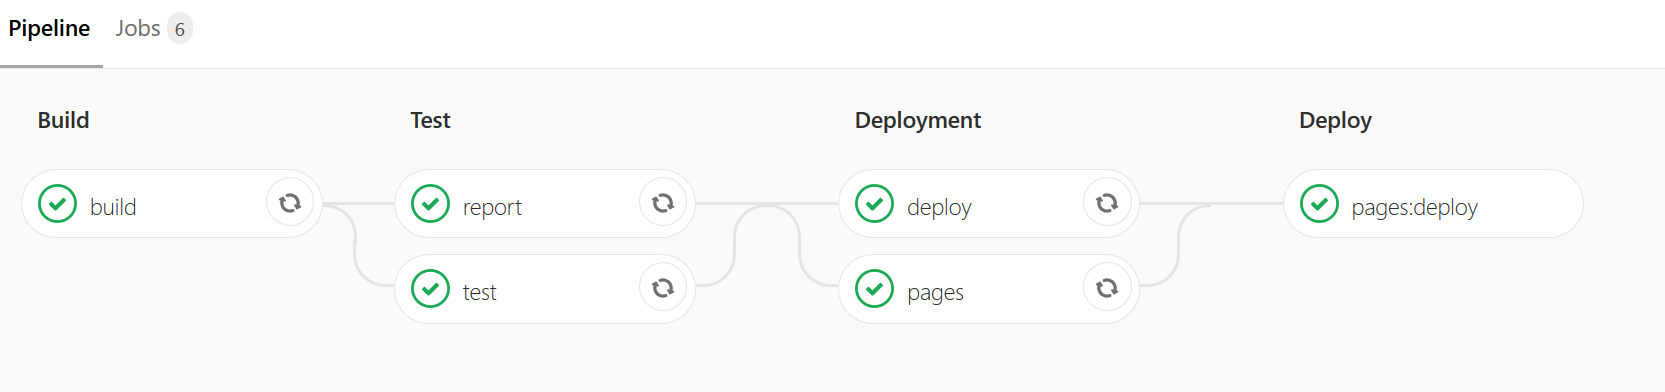
\includegraphics[width=0.9\textwidth]{M5_Pipeline}
 	\caption{Pipeline de GitLab que muestra éxito en todos los trabajos definidos para el proceso de CI/CD}\label{fig:M5_Pipeline}
 \end{figure}
 \FloatBarrier
 
 
 En la Fig. \ref{fig:M5_Pipeline_Error} se muestra un pipeline que dió error en la actividad de \textit{report} y, en consecuencia, se pasó por alto la actividad \textit{deploy}.
 
 \imagen{M5_Pipeline_Error}{Error en un pipeline}
%\todo añadir una captura de pantalla con el badge Heroku del  Readme de Gitlab y explicar como se actualiza cada vez que se realiza un commit. 
%\todo añadir una captura de pantalla con los check verdes en la lista de commit del repositorio de GitLab

\subsubsection{Tokens y variables de entorno}

Para llevar a cabo este proceso de CI/CD, ha sido necesario definir variables de entorno en GitLab que contienen las credenciales o tokens de acceso a Heroku y a Codacy. Esto se realiza desde la ventana de Configuración-CI/CD en la parte de `\textit{Variables}' como se muestra en la Fig. \ref{fig:M5_GitLab_Variables}.

\imagen{M5_GitLab_Variables}{Variables del entorno de ejecución de GitLab}

En el apartado anterior se vé un fragmento de código en el que se utilizan dos de las tres variables que se han definido y se ven en la Fig. \ref{fig:M5_GitLab_Variables}: \textit{\$CODACY\_PROJECT\_TOKEN} y \textit{\$CODACY\_API\_TOKEN}. La otra variable (\textit{HEROKU\_API\_KEY}) se utiliza indirectamente en la actividad de \textit{deploy} de la etapa de \textit{deployment}. Esta no se muestra en el script que define la actividad, sin embargo, fallaría la ejecución de la actividad si no se hubiera definido esta variable.

Estos tokens permiten conectarse a herramientas como Codacy o Heroku ya sea para iniciar sesión o para acceder directamente a un proyecto definido dentro de esas herramientas sin necesidad de tener que tener que iniciar sesión manualmente mediante usuario y contraseña. Esto permite automatizar las tareas que requieran iniciar sesión en herramientas de este tipo. Por ejemplo \textit{\$CODACY\_PROJECT\_TOKEN} es el token que permite acceder al proyecto correspondiente en Codacy y \textit{\$CODACY\_API\_TOKEN} permite utilizar Codacy con una sesión sin tener que iniciar sesión. El primero se obtuvo al configurar la cobertura de código en Codacy y el segundo desde la configuración de la cuenta de usuario en Codacy, en la pestaña `\textit{API Tokens}', se puede generar varios.

\subsubsection{Badges}

Los badges son distintivos o placas que se agregan el el fichero \textit{README} o en el lugar que se permita (admiten varios formatos como Markdown, HTML, Textile, AciiDoc, etc) y aportan información sobre el estado de ciertas características del proyecto tras el último commit como el resultado del pipeline de una actividad de CI/CD, la revisión de calidad, la revisión de cobertura, el estado del despliegue, etc.

En la Fig. \ref{fig:M5_GitLab_Badges_Readme} se muestran los badges que se han definido en el fichero README.md del proyecto. Los badges constan de tres partes:
\begin{itemize}
	\tightlist
	\item Nombre del badge
	\item Imagen en formato \textit{.svg} asociada al estado del atributo que evalúa el badge y ofrecida por el proveedor de la información
	\item Enlace al que redirige al clicar sobre él. Normalmente una página que complete la información que ofrece el badge.
\end{itemize}
En Markdown la sintaxis es la siguiente:

\begin{minipage}{\linewidth}
{\tiny
\begin{lstlisting}[breaklines]
...
[![nombre-del-badge](URL-de-la-imagen)](URL-del-link)
...		
\end{lstlisting}
}
\end{minipage}
, mientras que en HTML sería:

\begin{minipage}{\linewidth}
{\tiny
\begin{lstlisting}[breaklines]
...
<a href="URL-del-link"><img src="URL-de-la-imagen"/></a>
...		
\end{lstlisting}
}
\end{minipage}

\imagen{M5_GitLab_Badges_Readme}{Badges definidas en el fichero README.md del repositorio del proyecto}

En el proyecto se han definido cuatro badges:
\begin{itemize}
	\item \textit{\textbf{Pipeline}}. Muestra la información del último \textit{pipeline} del proyecto ejecutado en GitLab: en ejecucion (\textit{running}), ejecutado correctamente (\textit{passed}), o ejecutado con fallos (\textit{failed}). El proveedor de la imagen y de la información es GitLab y enlaza con el último \textit{pipeline} del proyecto.
	
	\item \textit{\textbf{Code Quality}}. Muestra la calificación de calidad de código que da Codacy al proyecto y enlaza a la página del proyecto en Codacy.
	
	\item \textit{\textbf{Coverage}}. Muestra el porcentaje de cobertura de instrucciones de las pruebas que se realizan durante la ejecución del \textit{pipeline} de GitLab y enlaza a la página del proyecto en Codacy. El dato es recogido durante la actividad \textit{report} de la fase de \textit{test} del \textit{pipeline}.
	
	\item \textit{\textbf{Coverage}}. Debido a problemas con Codacy, se ha decidido poner otro badge de cobertura. Esta vez se obtiene la información directamente desde el pipeline del último commit del repositorio del proyecto. Y enlaza a un informe que genera JaCoCo en formato HTML y que es publicado en el mismo repositorio del proyecto.
\end{itemize}

\subsection{Pruebas unitarias automáticas con JUnit y GitLab}

Para la automatización de la fase de pruebas se han utilizado las herramientas JUnit, Maven y los \textit{pipelines} GitLab.

\subsubsection{Desarrollo de las pruebas con JUnit}

JUnit es un framework que permite desarrollar pruebas unitarias sobre el código desarrollado. Además, dispone de un motor para la ejecución de las pruebas y la visualización de los resultados. En este proyecto se ha utilizado JUnit 5. Esta es la última versión de JUnit y permite, entre otras cosas:
\begin{itemize}
	\item Realizar asertos (\textit{asserts}) de tipo \textit{\textbf{assertAll()}} \footnote{\url{https://junit.org/junit5/docs/current/api/org/junit/jupiter/api/Assertions.html}}. Se realizó en pruebas en versiones previas de la aplicación pero se optó por quitarlos y utilizar asertos simples.
	
	\item Realizar \textbf{comprobaciones de lanzamiento de excepciones} en asertos del tipo \textit{assertThrows()}. De esta forma se pueden comprobar todos los casos de pruebas, tanto aquellos en los que se espere un resultado como aquellos en los que se debería lanzar una excepción. Por ejemplo, un test que espera una excepción sería:\\
\begin{minipage}{\linewidth}
{\tiny
\begin{lstlisting}[breaklines]
...
@ParameterizedTest(name = "Run with User = \"{0}\" and Password = \"{1}\" must throw an exception.")
@CsvFileSource(resources = "/testConnectUserPasswordWrong.csv", numLinesToSkip = 1, delimiter = ';', encoding = "UTF-8")
public void testConnectUserPasswordWrong(String user, String password) {
  assertThrows(RepositoryDataSourceException.class, () -> {
	repositoryDataSource.connect(user, password);
  }, getErrorMsg("testConnectUserPasswordWrong", "Wrong user-password should throw an exception"));
  assertEquals(EnumConnectionType.NOT_CONNECTED, repositoryDataSource.getConnectionType(), getErrorMsg("testConnectUserPasswordWrong", "Connection type must be 'NOT_CONNECTED'"));
}
...		
\end{lstlisting}
}
\end{minipage}
	
	Este comprueba que tras ejecutar la función con un conjunto de combinaciones posibles de usuario y contraseña incorrectos como argumentos, se lance una excepción y se mantenga un estado consistente en un objeto de la clase \textit{RepositoryDataSource}.
	
	\item Permite crear \textbf{test parametrizados}. Estos son test que prueban funciones que requieren argumentos y cada combinación de argumentos es un caso de prueba. 
	
	Crear un test para cada combinación es un caso claro del defecto de código: `código duplicado' y dificultan la mantenibilidad del proyecto. Por ello estos argumentos se pueden generar mediante funciones, enumeraciones, proveedores de argumentos o recolectar desde un CSV y solo ser necesario un test para todas las combinaciones de argumentos posibles. Otra ventaja de poder realizar pruebas parametrizadas es que el mismo \textit{CSV} sirve para diferentes funciones de pruebas.
	
	Para poder parametrizar los test es necesario agregar una dependencia adicional al proyecto \textit{junit-jupiter-params} junto con la dependencia del API de JUnit \textit{junit-jupiter-api}.
	
	Un ejemplo de estos se encuentra en el código anterior, que tiene la anotación \textit{@ParameterizedTest} y recibe los argumentos de un fichero \textit{CSV} ubicado en \textit{src/test/resources} y llamado \textit{testConnectUserPasswordWrong.csv} que contiene los datos de prueba:\\
\begin{minipage}{\linewidth}
{\tiny
\begin{lstlisting}[breaklines]
USER;PASSWORD
;a
a;
;
"";a
a;""
"";""
mlb0029;a	
\end{lstlisting}
}
\end{minipage}
	
	Cada columna del CSV es un argumento de la función. La diferencia entre poner comillas dobles y no poner nada es escribir un \textit{String} vacío o \textit{null}, respectivamente. La primera linea es la cabecera para mejorar la comprensión del \textit{CSV}. Para no contar esa linea como argumentos, se debe configurar la anotación \textit{@CsvFileSource} con 
\begin{minipage}{\linewidth}
{\tiny
\begin{lstlisting}[breaklines]
numLinesToSkip = 1
\end{lstlisting}
}
\end{minipage} 
como se puede observar en el código del punto anterior.
		
	\item Permite realizar presunciones (\textit{\textbf{assumptions}}) que permiten realizar una comprobación que pasará por alto el test sin marcarla como error (lo marca como \textit{skipped}) si la comprobación falla. 
	
	Esto ha sido útil de cara a probar funciones que realicen conexiones a GitLab que requieran credenciales de acceso. No es correcto escribir en el código las credenciales de acceso. Por tanto estos test tienen presunciones que comprueban si se tienen las credenciales de acceso (p.ej en un fichero o en variables auxiliares). Estos test se ejecutan en tiempo de desarrollo con las credenciales que aporta el equipo de desarrollo y no se ejecutan automáticamente en el proceso de integración continua de GitLab. En lugar de lanzar un error por no tener las credenciales, los test se pasan por alto y no se ejecutan.
\end{itemize}

\subsubsection{Proyectos de pruebas}

Para realizar pruebas en la obtención de información de repositorios de GitLab se han creado dos proyectos de pruebas (uno privado y otro público) y se ha utilizado otro adicional importado desde GitHub de uno de los trabajos para una asignatura:
\begin{itemize}
	\tightlist
	\item \url{https://gitlab.com/mlb0029/privatetestproject}
	\item \url{https://gitlab.com/mlb0029/publictestproject}
	\item \url{https://gitlab.com/mlb0029/ListaCompra}
\end{itemize}
Se han realizado commits e issues en los proyectos que se han creado para probar las funciones que obtienen información de GitLab. Estos datos se han almacenado en ficheros \textit{CSV} para poder parametrizar las pruebas (ver Fig. \ref{fig:M5_CSV_ProyectosPruebas}).

\imagen{M5_CSV_ProyectosPruebas}{Datos de proyectos de pruebas en fichero CSV}

\subsubsection{Automatización de las pruebas}

Para automatizar el proceso de pruebas se ha utilizado Maven y los \textit{pipelines} de GitLab.

Para ello se debe incluir una dependencia al proyecto: \textit{junit-jupiter-engine} que es el motor de ejecución de pruebas de JUnit. Y en el \textit{build} incluir los siguientes plugins:\\
\begin{minipage}{\linewidth}
{\tiny
\begin{lstlisting}[breaklines]
  <!-- Unit tests -->
  <plugin>
	<groupId>org.apache.maven.plugins</groupId>
	<artifactId>maven-surefire-plugin</artifactId>
	<configuration>
	  <reportsDirectory>${project.reporting.outputDirectory}/surefire-reports</reportsDirectory>
	</configuration>
	<version>2.22.1</version>
  </plugin>
  <!-- Integration tests -->
  <plugin>
	<groupId>org.apache.maven.plugins</groupId>
	<artifactId>maven-failsafe-plugin</artifactId>
	<version>2.22.1</version>
  </plugin>	
\end{lstlisting}
}
\end{minipage}

Con esto, se puede ejecutar \textit{mvn test} para ejecutar las pruebas. Este comando puede ser agregado en una de las actividades del fichero \textit{.gitlab-ci.yml} para ejecutar las pruebas automáticamente al hacer un commit en GitLab. Por ejemplo, la actividad \textit{test} de la fase \textit{test}:\\
\begin{minipage}{\linewidth}
{\tiny
\begin{lstlisting}[breaklines]
...
test:
  stage: test
  script:
	- mvn test
...
\end{lstlisting}
}
\end{minipage}

\subsection{Pruebas con Tomcat}

Desde que se empezó ha implementar la interfaz. Se configuró un entorno Tomcat en el que poder desplegar la aplicación y visualizar y probar los elementos de la interfaz gráfica.

Para realizar esto se instaló Tomcat en el equipo local del programador y se configuró la correspondiente variable de entorno del sistema \textit{CATALINA\_HOME} con la ruta a la carpeta de instalación. Conviene, también, tener definida la variable \textit{JAVA\_HOME} apuntando al directorio de instalación del JDK (o JRE) de Java.

Como \textit{Eclipse IDE for Java EE Developers} y Tomcat se integran muy bien, se puede configurar un servidor Tomcat con Eclipse desde la vista \textit{Servers}. Solo hay que elegir la versión de Tomcat (la 9 para Java 11) y especificar: el nombre del servidor, el directorio de instalación de Tomcat y el JRE a utilizar (Java 11). Una vez hecho esto se puede desplegar la aplicación desde eclipse fácilmente (\textit{Run As/Run on Server}), siempre que el puerto 8080 que usa Tomcat esté disponible y el servidor arrancado. Se puede acceder a la aplicación desde el navegador con la url: 
\begin{minipage}{\linewidth}
{\tiny
\begin{lstlisting}[breaklines]
http://localhost:8080/[nombre-proyecto]
\end{lstlisting}
}
\end{minipage}
y probar la aplicación en distintos navegadores.

También se puede hacer sin Eclipse. Para ello, solo basta con tener el puerto 8080 disponible y ejecutar en una consola de comandos el comando \textit{startup}. Se arrancará el servidor Tomcat. Antes conviene configurar un usuario de Tomcat con rol `\textit{manager-gui}' desde el fichero
\begin{minipage}{\linewidth}
{\tiny
\begin{lstlisting}[breaklines]
$CATALINA_HOME/conf/tomcat-users.xml
\end{lstlisting}
}
\end{minipage}
. Por ejemplo:\\
\begin{minipage}{\linewidth}
{\tiny
\begin{lstlisting}[breaklines]
...
<role rolename="manager-gui"/>
<user username="blah" password="blah" roles="manager-gui"/>
...
</tomcat-users>
\end{lstlisting}
}
\end{minipage}
Una vez arrancado Tomcat, se puede acceder desde el navegador a \textit{http://localhost:8080} (aparecerá una ventana similar a la de la Fig. \ref{fig:M5_Tomcat_Main}) y pulsar sobre \textit{Manager App}. Desde el gestor de aplicaciones se pueden desplegar varias aplicaciones, publicando el fichero \textit{.war} de la aplicación.

\imagen{M5_Tomcat_Main}{Ventana principal de la GUI de Tomcat}

Cada vez que se añadía un elemento a la interfaz se realizaban pruebas y se cuadraba el elemento dentro de la interfaz. Una vez que se creaba una funcionalidad completa, también se realizaban pruebas sobre la interfaz. Por ejemplo, añadir un repositorio o calcular las métricas. Para las pruebas se disponían de datos de otros repositorios de GitLab que se han presentado como TFG en el Grado de Ingeniería Informática en la Universidad de Burgos. Esto ha facilitado en gran medida el trabajo de pruebas. Es destacable la funcionalidad de acceso a los repositorios por el concepto de grupo definido en Gitlab. Esto fue posible gracias a que la empresa Hewlett Packard SCDS en su colabaración con TFGs con la UBU organiza sus propuestas de TFGs en GitLab en grupos para organizarlos por cursos académicos.

\subsection{Revisión automática de la cobertura con Codacy}

La cobertura es el porcentaje de la aplicación que se ha probado. Esto se puede medir en relación a lineas de código, instrucciones, clases, bifurcaciones (condicionales y bucles) y métodos. Lo normal es mostrar la cobertura de instrucciones.

Para realizar las revisiones automáticas de cobertura, lo primero que hay que hacer es definir las pruebas y ejecutarlas. Como este proceso se ha explicado anteriormente, se procede a describir el proceso de cobertura.

Las revisiones automáticas de cobertura se han realizado utilizando JaCoCo, Codacy y GitLab. Sin embargo, JaCoCo es el que genera los informes que se envían tanto a Codacy como a GitLab.

\subsubsection{Configuración de JaCoCo con Maven}

Antes que nada se ha añadido una sección en el fichero pom.xml:\\
\begin{minipage}{\linewidth}
{\tiny
\begin{lstlisting}[breaklines]
...
<reporting>
  <outputDirectory>${project.build.directory}/reports</outputDirectory>
</reporting>
...
\end{lstlisting}
}
\end{minipage}
en la que se define el directorio dónde se generarán todos los informes (incluidos los informes de las pruebas). Y en la sección de \textit{build} se añade el siguiente plugin de la siguiente manera:\\
\begin{minipage}{\linewidth}
{\tiny
\begin{lstlisting}[breaklines]
...
<plugin>
  <groupId>org.jacoco</groupId>
  <artifactId>jacoco-maven-plugin</artifactId>
  <version>0.8.3</version>
  <configuration>
	<outputDirectory>${project.reporting.outputDirectory}/jacoco-reports</outputDirectory>
	<output>file</output>
	<title>Coverage of project: ${project.name}</title>
  </configuration>
</plugin>
...
\end{lstlisting}
}
\end{minipage}
En la configuración se define el directorio de destino de los informes, que se desea que se generen en forma de fichero y se define el título del fichero. De esta forma, se puede generar los informes con Maven de la siguiente manera:\\
\begin{minipage}{\linewidth}
{\tiny
\begin{lstlisting}[breaklines]
$ mvn clean jacoco:prepare-agent install jacoco:report
$ mvn jacoco:report
\end{lstlisting}
}
\end{minipage}

El primer comando genera el fichero \textit{jacoco.exec} que es necesario para la ejecución del segundo comando.

\subsubsection{Configuración de Codacy}

Codacy permite llevar una revisión de la calidad de código y de la cobertura de las pruebas.

Para utilizar esta herramienta se debe tener una cuenta. Permite iniciar sesión con GitHub, Bitbucket o Google. Una vez iniciada sesión permite añadir proyectos al entorno Codacy. Para añadir proyectos se debe pulsar sobre el botón \textit{Add project} como se muestra en la Fig. \ref{fig:M5_Codacy_ProjectsPage}. Se pueden importar los proyectos desde GitHub o Bitbucket (hay que solicitar permisos a GitHub o Bitbucket). Nada más añadirlos, realiza un análisis inicial de la calidad de código y, posteriormente, realizará este análisis cada vez que se realice un \textit{commit} en GitHub o Bitbucket.

\imagen{M5_Codacy_ProjectsPage}{Página principal de Codacy para la gestión de proyectos}

Para configurar la revisión de cobertura hay que seguir unos pasos más. Desde la página de \textit{Dashboard} del proyecto (ver Fig. \ref{fig:M5_Codacy_Dashboard}) se puede observar el indicador de cobertura con título \textit{Coverage}. En un proyecto nuevo, este indicador no está disponible hasta que se haya configurado la cobertura, en su lugar aparece el siguiente mensaje: ``\textit{Make sure your code is all tested. Set up your coverage here.}'' con un enlace. El enlace lleva a una página que contiene: el token del proyecto e instrucciones a seguir según el lenguaje de programación.

\imagen{M5_Codacy_Dashboard}{Vista Dashboard del proyecto en Codacy}

Para este proyecto, la configuración de cobertura de Codacy se ha realizado de la siguiente manera:
\begin{enumerate}
	\item Es importante copiar el token del proyecto que se muestra en la página de instrucciones mencionada anteriormente. 
	
	\item Configurar el plugin JaCoCo como se ha indicado anteriormente.
	
	\item Utilizar \textit{codacy-maven-plugin} para enviar el informe de cobertura generado por JaCoCo a Codacy. También se puede añadir el plugin en la sección de \textit{buid} del \textit{pom.xml}:\\
\begin{minipage}{\linewidth}
{\tiny
\begin{lstlisting}[breaklines]
<plugin>
  <groupId>com.gavinmogan</groupId>
  <artifactId>codacy-maven-plugin</artifactId>
  <version>1.2.0</version>
  <configuration>
	<coverageReportFile>${project.reporting.outputDirectory}/jacoco-reports/jacoco.xml</coverageReportFile>
  </configuration>
</plugin>
\end{lstlisting}
}
\end{minipage}
	En la configuración se le indica la ubicación del fichero que debe enviar a Codacy.

	\item Para enviar el informe de cobertura se tendrá que generar los informes de JaCoCo con los comandos Maven del apartado anterior y ejecutar el siguiente comando:\\
\begin{minipage}{\linewidth}
{\tiny
\begin{lstlisting}[breaklines]
$ mvn com.gavinmogan:codacy-maven-plugin:coverage -DprojectToken="$CODACY_PROJECT_TOKEN" -DapiToken="$CODACY_API_TOKEN"
\end{lstlisting}
}
\end{minipage}
	Siendo \textit{\$CODACY\_PROJECT\_TOKEN} el token del proyecto del que se habla en el primer punto y \textit{\$CODACY\_API\_TOKEN} el token de usuario poara utilizar el API de Codacy. Este último se obtiene desde la gestión de la cuenta de usuario.
\end{enumerate}

\subsubsection{Configuración de GitLab}

Se ha configurado JaCoCo y el plugin para enviar los informes de JaCoCo a Codacy para realizar estas actividades con comandos Maven. Pero para automatizar este proceso se deben añadir las actividades correspondientes al flujo de trabajo de CI/CD de GitLab, es decir: el fichero \textit{.gitlab-ci.yml}.

Para ello se ha definido la actividad \textit{report} en la etapa de \textit{test}, ejecutando los comandos Maven  con unas pequeñas modificaciones:\\
\begin{minipage}{\linewidth}
{\tiny
\begin{lstlisting}[breaklines]
report:
  stage: test
  script:
	- mvn clean jacoco:prepare-agent install jacoco:report
	- mvn jacoco:report -DdataFile=$CI_PROJECT_DIR/target/jacoco.exec
	- mvn com.gavinmogan:codacy-maven-plugin:coverage -DprojectToken="$CODACY_PROJECT_TOKEN" -DapiToken="$CODACY_API_TOKEN"
  artifacts:
	paths:
	  - $CI_PROJECT_DIR/target/reports/jacoco-reports/
\end{lstlisting}
}
\end{minipage}
\begin{itemize}
	\item En el segundo comando se añade la opción \textit{-DdataFile} que indica la ubicación del fichero \textit{jacoco.exec} que se genera en el entorno de GitLab.
	\item Para utilizar \textit{\$CODACY\_PROJECT\_TOKEN} y \textit{\$CODACY\_API\_TOKEN} se deben configurar las variables de entorno de GitLab como se indica en la sección `Tokens y variables de entorno'.
	\item Se ha añadido \textit{artifacts} con la ruta que apunta al directorio que contiene los informes de JaCoCo definido en Maven (ver `Configuración de JaCoCo con Maven'). Con esto se agrega este directorio a los artefactos de la actividad.
\end{itemize}

La parte de \textit{artifacts} no tiene que ver con JaCoCo ni con Codacy. Entonces, ¿por qué añadirlo? 

Codacy tenía demasiados problemas al soportar GitLab y otras forjas de repositorios (añadir proyecto a Codacy con \textit{Git URL}) y decidieron eliminar esta funcionalidad. Por tanto, cesaron las revisiones automáticas de calidad y cobertura. Para solucionar esto se puede exportar a GitHub el proyecto y añadir el proyecto a Codacy impostándolo desde GitHub. Sin embargo, se deseaba seguir trabajando con GitLab. Una solución es hacer un \textit{Git push} tanto para GitLab como para GitHub cada vez que se realice un commit y en GitLab añadir los badges y las variables de entorno que enlazan al proyecto en Codacy, pero que realmente es importado desde GitHub.

Adicionalmente, se estudio la forma de agregar la cobertura directamente desde GitLab. Puesto que se podía hacer, pero al disponer de Codacy, se opto por utilizar Codacy. Entonces se puede publicar directamente el informe de JaCoCO en formato \textit{HTML} en GitLab y añadir un badge de Cobertura. Para ello, se debe generar el informe con formato HTML en una de las actividades y almacenarlo en los artefactos de la actividad. Esta es la explicación de \textit{artifacts}. Posteriormente se publican estos artefactos en las páginas del proyecto en GitLab (\textit{Settings - Pages}). Lo mejor sería añadir el enlace al informe en el README del proyecto y qué mejor forma que añadirlo en forma de badge. 

Para agregar el badge, se necesita mostrar en un log de las actividades un informe de cobertura donde venga el porcentaje total: el fichero \textit{index.html} generado por JaCoCO tiene este dato. Lo que falta es añadir la expresión regular que lo identifica en el fichero en la configuración del proyecto (Settings - CI/CD -  General pipelines) en la parte de `Test coverage parsing'. La expresión regular es la siguiente para ese fichero:\\
\begin{minipage}{\linewidth}
{\tiny
\begin{lstlisting}[breaklines]
/<td>Total<\/td><td class="bar">\d{1,3}(,\d{1,3})? of \d{1,3}(,\d{1,3})?<\/td><td class="ctr2">(\d{1,3})%<\/td>/
\end{lstlisting}
}
\end{minipage}
Si se muestra el informe en el log de las actividades de un \textit{pipeline}, y se ha definido bien la expresión regular, desde \textit{Settings - CI/CD -  General pipelines} se muestran tanto el badge del estado del \textit{pipeline} como el de cobertura (ver Fig. \ref{fig:M5_GitLab_Badges_CoverageAndPipeline}). Solo queda añadirlos al fichero README y/o a los badges del proyecto como se indica en la sección `Badges'. Se recomienda cambiar el enlace del badge del informe de cobertura por el enlace al informe de cobertura de JaCoCO publicado en las \textit{Pages} del proyecto.

\imagen{M5_GitLab_Badges_CoverageAndPipeline}{Configuración de CI/CD de GitLab: Pipeline status and Coverage report}

La publicación del informe y mostrar en el log el fichero \textit{index.html} se realiza en la actividad \textit{pages} de la fase \textit{deployment} de la siguiente manera:\\
\begin{minipage}{\linewidth}
{\tiny
\begin{lstlisting}[breaklines]
...
pages:
  stage: deployment
  dependencies: 
	- report
  script:
	- cat $CI_PROJECT_DIR/target/reports/jacoco-reports/index.html
	- mv $CI_PROJECT_DIR/target/reports/jacoco-reports/ public/
  artifacts:
	paths:
	  - public
	expire_in: 30 days    
  only:
	- master
...
\end{lstlisting}
}
\end{minipage}

Con el comando cat se visualiza en el log el fichero \textit{index.html} y con el comando mv de publican los documentos HTML del informe de cobertura. También se almacenan los artefactos del directorio \textit{public} en el \textit{pipeline} durante 30 días. Y se ha configurado para que la actividad solo se haga al realizar cambios en la rama \textit{master} si la actividad \textit{report} se ha ejecutado sin problemas.

\subsection{Administración de calidad automática con Codacy}

Ya se ha mencionado en la sección `Configuración de Codacy' que este realiza revisiones automáticas de calidad y como se configura para ello, siendo un proceso bastante sencillo. Esto permite analizar la deuda técnica y, en caso de ser necesario, definir tareas para disminuir esta deuda. 

La valoración final del proyecto ha sido la máxima (A). Esta se muestra en el badge de `Code Quality', como se puede ver en la Fig. \ref{fig:M5_GitLab_Badges_Readme}. Al pulsar sobre el badge, se abre una pestaña en el navegador al proyecto en Codacy (\url{https://app.codacy.com/manual/mlb0029/comparador-de-metricas-de-evolucion-en-repositorios-software/dashboard}), como se muestra en la Fig. \ref{fig:M5_Codacy_Dashboard_Complete}.

\imagen{M5_Codacy_Dashboard_Complete}{Dashboard del proyecto en Codacy}

Este muestra la evolución en el tiempo de y una vista del estado actual de: el porcentaje de problemas de calidad (4\%), la complejidad de los ficheros (0\%), el código duplicado (0\%) y la cobertura (si se ha configurado) (18\%). Este gráfico ha ayudado a lo largo del desarrollo de la aplicación a valorar la evolución de la deuda técnica. En momentos de crecimiento, se puede ir a la ventana `Issues'  y ver los defectos de diseño que causan el aumento de la deuda (ver Fig. \ref{fig:M5_Codacy_Issues}). Se muestran los problemas por fichero y se muestra la linea de código que se debe corregir para disminuir la deuda técnica.

\begin{figure}[!h]
	\centering
	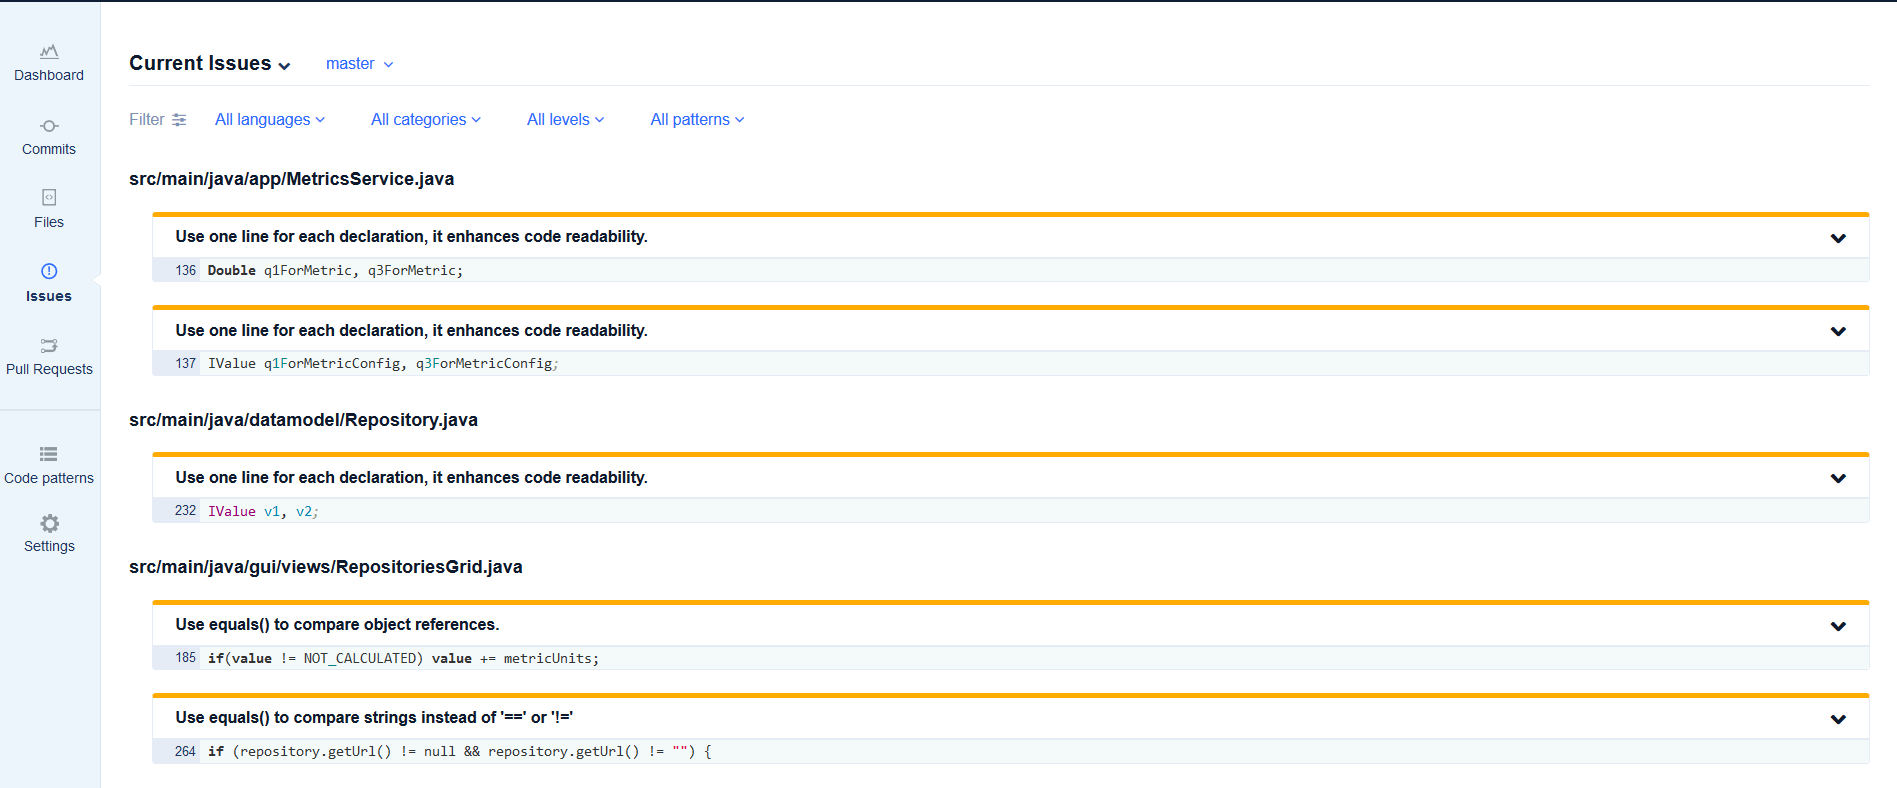
\includegraphics[width=1.0\textwidth]{M5_Codacy_Issues}
	\caption{Ventana Issues de Codacy con defectos que causan aumento de la deuda técnica}\label{fig:M5_Codacy_Issues}
\end{figure}
\FloatBarrier

Al gestionar la revisión de calidad por primera vez en este proyecto, Codacy permitía añadir repositorios a partir de su \textit{Git URL}. Esto permitió añadir nuestro proyecto de GitLab al entorno de Codacy. Sin embargo, esta funcionalidad les daba muchos problemas y la acabaron eliminando. Esto paró las revisiones de calidad automáticas de este proyecto. Para solucionar este problema se ha exportado el proyecto a GitHub y se ha añadido a Codacy desde GitHub para realizar una revisión final, con el código ya creado. Es por esta razón que no se aprecia la evolución en la Fig. \ref{fig:M5_Codacy_Dashboard_Complete}. 

\subsection{Despliegue automático con Heroku}

\subsubsection{Configuración de la Herramienta Heroku}

Heroku es una plataforma que permite desplegar una aplicación web en sus servidores. Para ello debes tener una cuenta, crear un pipeline y una aplicación y asociar la aplicación al pipeline. Para desplegarla se ofrecen tres opciones: \textit{Heroku Git}, \textit{GitHub} y \textit{Heroku CLI}.

En este proyecto se ha utilizado Heroku CLI y un plugin para integrarlo con Maven:\\
\begin{minipage}{\linewidth}
{\tiny
\begin{lstlisting}[breaklines]
...
<plugin>
  <groupId>com.heroku.sdk</groupId>
  <artifactId>heroku-maven-plugin</artifactId>
  <version>2.0.9</version>
  <configuration>
	<appName>evolution-metrics</appName>
  </configuration>
</plugin>
...
\end{lstlisting}
}
\end{minipage}

En el código anterior se configura el plugin para desplegar en la aplicación con nombre \textit{evolution-metrics}. El comando para  desplegar la aplicación sería \textit{\$ mvn clean heroku:deploy-war}. Sin embargo, para que funcione correctamente se debe iniciar sesión con \textit{\$ heroku login}, que abre el navegador en la página de inicio de sesión de Heroku. De esta forma es imposible desplegar la aplicación automáticamente, para hacerlo de una forma completamente automática se debe configurar la variable de entorno \textit{HEROKU\_API\_KEY} con el token de acceso \textit{API Key} que se obtiene desde la configuración de la cuenta de usuario de Heroku. Esta variable se ha definido dentro de las variables de entorno de GitLab de las que se hablaba anteriormente, y el comando de despliegue se ejecuta desde los \textit{pipelines} gracias a la actividad \textit{deploy} de la etapa \textit{deployment} definidas en el fichero \textit{.gitlab-ci.yml}.

\section{API de GitLab}

GitLab ofrece un API \footnote{\url{https://docs.gitlab.com/ee/api/}} REST \footnote{Representational state transfer} para poder desarrollar aplicaciones que integren funcionalidades de GitLab. En este proyecto se ha utilizado este API para establecer una conexión a GitLab y poder calcular métricas de los repositorios que aloje. Sin embargo, en lugar de trabajar directamente con GitLab REST API, se decidió usar un API en Java que permita operar con las características de GitLab REST API desde Java. Se encontraron dos proyectos en GitHub que implementan este tipo de APIs:
\begin{itemize}
	\tightlist
	\item \textit{timols/java-gitlab-api} \footnote{\url{https://github.com/timols/java-gitlab-api}}. 
	\item  \textit{gitlab4j/gitlab4j-api} \footnote{\url{https://github.com/gitlab4j/gitlab4j-api}}.
\end{itemize}

La primera impresión al entrar en \textit{timols/java-gitlab-api} es que el fichero \textit{README} está bastante vacío, tan solo contiene una descripción de lo que es y un enlace a la documentación. Al entrar en la documentación se puede observar que el código no está muy bien documentado, faltan muchas descripciones de funciones. Por estas razones, el coste de aprendizaje del API es muy alto y casi incomprensible. Además, tiene bastantes \textit{issues} abiertas y la última \textit{release} es de octubre de 2018, por lo que parece que la evolución del proyecto es lenta o a cesado.

Por el lado contrario, \textit{gitlab4j/gitlab4j-api} tiene un fichero \textit{README} explicativo, con índice de contenidos y muchos ejemplos. La documentación también tiene muchos elementos sin comentar, pero si que se ha documentado gran parte del sistema. El proyecto tiene muy pocas issues abiertas y está en constante evolución, sacando tres o cuatro \textit{releases} al mes y evolucionando a la vez que GitLab REST API. Es por estos factores por los que se decidió usar este API como intermediario entre nuestra aplicación en Java y GitLab REST API. Para utilizar este API solo ha sido necesario incluirlo entre las dependencias del proyecto en el fichero \textit{pom.xml}. 

\section{Diseño extensible}

\section{Interfaz gráfica: Vadin}
-Ventajas e inconvenientes
-Ejemplo de uso
-Framework de pestañas de conexión y gestión de repos
-Configuración en maven adicional para poder ser utilizado en internet explorer
-Díalogo: problemas y solución
-Designer
-Despliegue en tomcat, falta de xml, porque no jetty
-No Adaptativo
\capitulo{6}{Trabajos relacionados}

%Este apartado sería parecido a un estado del arte de una tesis o tesina. En un trabajo final grado no parece obligada su presencia, aunque se puede dejar a juicio del tutor el incluir un pequeño resumen comentado de los trabajos y proyectos ya realizados en el campo del proyecto en curso.
\section{Activiti-Api}

\epigraph{Aplicación que permite realizar un estudio del estado de un proyecto en GitHub mediante distintas métricas de evolución. Permitiendo tener una visión del ritmo de trabajo del proyecto, duración, numero de participantes y actividad.}{dba0010/Activiti-Api}

\begin{figure}[!h]
	\centering
	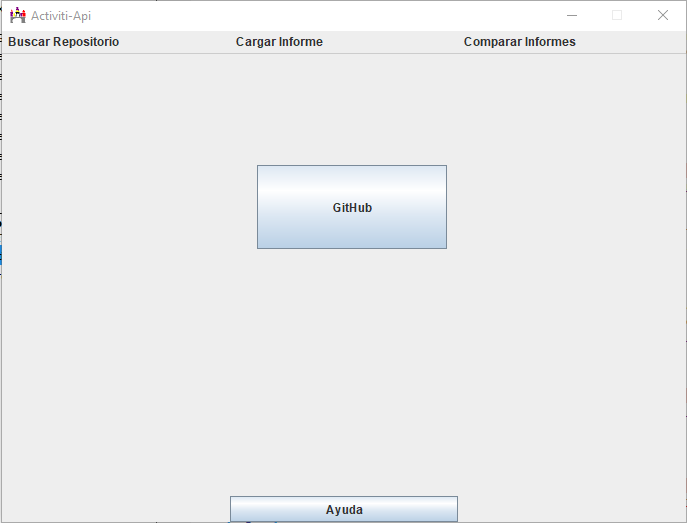
\includegraphics[width=0.65\textwidth]{M6_ActivitiApi_Ppal}
	\caption{Ventana principal de Activiti-Api}\label{fig:M6_ActivitiApi_Ppal}
\end{figure}

En un proyecto bastante parecido implementado como aplicación de escritorio escrita en lenguaje Java. En algunos aspectos ha sido modelo para el desarrollo de este proyecto software. Esta alojado en GitHub\footnote{\url{https://github.com/dba0010/Activiti-Api}} y se puede obtener y ejecutar. Se muestra la ventana principal en la Fig. \ref{fig:M6_ActivitiApi_Ppal}.

El aspecto que más llamó la atención para este proyecto es la forma de buscar repositorios. Permite establecer una conexión a GitHub iniciando sesión mediante usuario y contraseña o entrar en ``Modo desconectado'', como se muestra en la Fig. \ref{fig:M6_ActivitiApi_Con}. Una vez establecida la conexión permite mostrar las métricas de evolución de un proyecto, para ello hay que indicar un usuario del cual se quiere obtener un proyecto y seleccionar el proyecto de un desplegable con los proyectos de ese usuario, ver Fig. \ref{fig:M6_ActivitiApi_Proyectos}.

\begin{figure}[!h]
	\centering
	\includegraphics[width=0.65\textwidth]{M6_ActivitiApi_Con}
	\caption{Conexión a GitHub mediante Activiti-Api}\label{fig:M6_ActivitiApi_Con}
\end{figure}

\begin{figure}[!h]
	\centering
	\includegraphics[width=0.65\textwidth]{M6_ActivitiApi_Proyectos}
	\caption{Selección de un proyecto para obtener las métericas en Activiti-Api}\label{fig:M6_ActivitiApi_Proyectos}
\end{figure}

\subsection{Comparando Activiti-Api con este proyecto}

A continuación se muestran las diferencias del producto software de ``Activiti-Api'' con el producto generado en ``Comparador de métricas de evolución en repositorios software''.

\subsubsection{Interfaz}

Es una aplicación de escritorio, mientras que en este proyecto se ha optado por implementar una aplicación web.

\subsubsection{Conexión}

Para obtener información de los proyectos, Activiti-Api permite establecer una conexión a GitHub mientras que este proyecto permite establecer conexión a GitLab. Aunque este proyecto permite extender la funcionalidad a otras forjas de repositorios como GitHub.

Activiti-Api permite dos tipos de conexión: iniciar sesión a GitHub mediante usuario y contraseña o ``Modo desconectado'' (establece una conexión pública). 

Este proyecto permite iniciar sesión a GitLab mediante usuario y contraseña o por uso de un token de acceso personal. Además también permite establecer una conexión pública o directamente trabajar sin conexión sobre la aplicación. Dependiendo de la conexión escogida se limitará la funcionalidad de la aplicación. Por ejemplo, sin conexión no es posible añadir repositorios. Además se muestra al usuario de la aplicación el tipo de conexión escogida en todo momento y la información de sesión iniciada en caso de que se haya iniciado sesión en GitLab.

\subsubsection{Gestión de proyectos y evaluación de métricas}

Activiti-Api solo permite trabajar con un proyecto al mismo tiempo o comparar dos proyectos. La comparación se ha definido de forma estática durante el desarrollo del proyecto, permaneciendo invariable en tiempo de ejecución.

Este proyecto permite añadir múltiples proyectos, evaluarlos y compararlos mediante el cálculo estadístico de cuartiles para hallar los valores umbrales de cada métrica. Por tanto la comparación puede ser dinámica a partir de los proyectos que se escojan para la comparativa, aunque también se han definido unos valores umbrales predefinidos a partir de unas estadísticas obtenidas de un conjunto de datos obtenidos a partir de TFGs y publicado en GitHub \footnote{\url{https://github.com/clopezno/clopezno.github.io/blob/master/agile_practices_experiment/DataSet_EvolutionSoftwareMetrics_FYP.csv}}. Este proyecto permite gestionar perfiles de métricas con diferentes umbrales para distintos contextos de aplicación.

Activiti-Api genera un informe con los resultados de las métricas de un proyecto, varios gráficos y permite generar un informe de comparativa entre dos proyectos. Mientras que este proyecto muestra los resultados de varios proyectos en forma de tabla.

\subsubsection{Mantenibilidad y extensibilidad}

Este proyecto ha preparado un  framework para poder extender la fuente de datos, es decir las forjas. Ha sido implementado para obtener datos desde GitLab, pero es fácilmente extensible a otras forjas como GitHub. Activiti-Api no permite esta extensibilidad e incluye demasiadas dependencias con GitHub API.

Ambos proyectos siguen la solución basada en frameworks propuesta en \textit{Soporte de Métricas con Independencia del Lenguaje para la Inferencia de Refactorizaciones} \cite{marticorena_soporte_2005}. El objetivo del \textit{framework} es la reutilización en la implementación del cálculo de métricas. De hecho, Activiti-Api ha servido de ejemplo para la implementación del motor de métricas de este trabajo.

\section{Soporte de Métricas con Independencia del Lenguaje para la Inferencia de Refactorizaciones}

De este trabajo se ha basado la construcción del subsistema ``motor de métricas'', como se puede ver en la sección \ref{sect:3_3_3_FrameworkMedicion}.

\section{Software Project Assessment in the Course of Evolution -  Jacek Ratzinger}

Es de este trabajo de donde se han obtenido las métricas de control con las que se trabaja en este proyecto. Hay una explicación detallada en el apartado \ref{sect:3_3_2_MetricasControl}.
\capitulo{7}{Conclusiones y Líneas de trabajo futuras}

%Todo proyecto debe incluir las conclusiones que se derivan de su desarrollo. Éstas pueden ser de diferente índole, dependiendo de la tipología del proyecto, pero normalmente van a estar presentes un conjunto de conclusiones relacionadas con los resultados del proyecto y un conjunto de conclusiones técnicas. 
%Además, resulta muy útil realizar un informe crítico indicando cómo se puede mejorar el proyecto, o cómo se puede continuar trabajando en la línea del proyecto realizado. 
\section{Conclusiones}
En este proyecto se ha aprendido a configurar una aplicación web en Java, realizar interfaces gráficas usando solo Java, configurar un proyecto de forma que se facilite la integración y despliegue continuos y la importancia que tiene para un equipo de desarrollo software, la importancia del uso de herramientas que midan la calidad de código, la importancia que tienen las métricas de proceso a la hora de gestionar un proyecto software, la comodidad y eficiencia que tienen las metodologías ágiles.
\section{Lineas de trabajo futuras}
Se definen en lista ideas que podrían realizarse en el futuro:
\begin{itemize}
	\item Extender la funcionalidad a nuevas métricas de evolución
	\item Extender las plataformas de desarrollo colaborativo a otras como GitHub, Bitbucket
	\item GitLab ofrece la posibilidad a los usuarios de tener su propia instancia de GitLab en un servidor propio. Por ahora solo se puede conectar al host ``https://gitlab.com/'', se podría ampliar esta funcionalidad permitiendo realizar una conexión a servidores propios
	\item Realizar un histórico de mediciones y almacenarlo en una base de datos
	\item Hacer que la aplicación web sea adaptable (\textit{responsive})
	\item Internacionalizar la aplicación
	\item Los proyectos y perfiles de métricas importados y exportados se almacenan en un buffer en memoria. Mientras el proyecto sea pequeño no hay problema, pero conforme vaya creciendo habría que implementar otros sistemas de persistencia como bases de datos o ficheros.
	\item Se podría permitir seleccionar varios proyectos de la tabla de la página principal para poder gestionar varios proyectos a la vez. Por ejemplo: crear un perfil de métricas sólo con los proyectos seleccionados, evaluar solo los proyectos seleccionados, eliminar varios proyectos a la vez, volver a obtener métricas de varios proyectos al mismo tiempo.
	\item La aplicación web solo soporta una sesión, se podría preparar para poder explotarlo en un entorno multisesión.
\end{itemize}


\bibliography{bibliografia}
\bibliographystyle{plainnat}

\end{document}
